% UoS Vitrine + DreamLab Object Sidecar — combined closeout report
% Engine: pdflatex (TeX Live 2025). Build: make (see Makefile).
% Sources for every figure/number are cited in-line as % SRC: comments.
\documentclass[10pt,twocolumn,a4paper]{article}

\usepackage[T1]{fontenc}
\usepackage[utf8]{inputenc}
\usepackage{lmodern}
\usepackage[british]{babel}
\usepackage[a4paper,margin=16mm,columnsep=6mm]{geometry}
\usepackage{microtype}
\usepackage{booktabs}
\usepackage{array}
\usepackage{graphicx}
\usepackage{caption}
\usepackage{subcaption}
\usepackage{xcolor}
\usepackage{amsmath}
\usepackage{siunitx}
\usepackage{enumitem}
\usepackage[hidelinks]{hyperref}
\usepackage{titlesec}

% Figures live in the sidecar/run tree, referenced read-only.
\graphicspath{{figures/}{../../runs/}{../../runs/nc04-object-pass1/}{../../runs/gallery-object-eval/}{figures/nc04-object-pass1/}{figures/gallery-object-eval/}{figures/nc04-generate-pass1/}{../../runs/nc04-generate-pass1/}}

% \todo{...} — a visible placeholder for content pending a run.
\newcommand{\todo}[1]{\textcolor{red}{\textbf{[TODO: #1]}}}

% Compact captions and headings for a dense two-column layout.
\captionsetup{font=small,labelfont=bf,skip=3pt}
\setlist{nosep,leftmargin=1.2em}
\titlespacing*{\section}{0pt}{6pt}{2pt}
\titlespacing*{\subsection}{0pt}{4pt}{1pt}
\sisetup{detect-weight=true,detect-family=true}

\setlength{\parskip}{2pt}
\setlength{\parindent}{0pt}

\title{\vspace{-8mm}\textbf{Archive-grade scene preservation and derived object
reconstruction: a combined closeout}\\[2pt]
\large Nested Cinema --- \textit{Vera's Not Alone}: UoS Vitrine scene pipeline and
the DreamLab object sidecar}

\author{Glenn Watts (UoS Vitrine, University of Salford)\\
DreamLab AI Consulting Ltd (object sidecar)\\[2pt]
\small Combined evidence to 28 August 2026}
\date{}

\begin{document}
\maketitle

% SRC: recovered-report/report.md Abstract (lines 12-20); object-sidecar PRD-001, VALIDATION.md, nc04-object-pass1/REPORT.md
\begin{abstract}
\small
This report closes an engagement that joins two systems around one artwork.
UoS Vitrine is a free, fully local pipeline that turns photographs and video of a
physical space into a 3D Gaussian splat, packaged with its source material, camera
solution, software record and checksums so the reconstruction can be treated as a
defensible preservation object. The DreamLab object sidecar is a separate repository
that consumes a sealed Vitrine run and derives per-object textured assets placed back
into the scene, with strict separation of observed evidence from generated proposal.
The test bed is \textit{Nested Cinema --- Vera's Not Alone}, Dr Pavel Prokopic's
immersive installation at the University of Salford, MediaCityUK.

The validated laptop scene run registered 222 of 222 images, trained one million
Gaussians in \SI{60.4}{\minute} on an RTX 3060 Laptop GPU, and reached
\SI{25.72}{\decibel} PSNR and 0.8167 SSIM on 28 held-out views at \SI{1.94}{\giga\byte}
peak VRAM. An RTX 5090 reproduction of the same recipe reached \SI{25.06}{\decibel} and
0.8211 SSIM in \SI{2.4}{\minute} --- matching laptop quality roughly 25 times faster.
A workstation-archive profile (1600-pixel crop from 4096-pixel sources) suffered mass
opacity collapse and is quarantined as an unvalidated negative result.

The object sidecar runs end-to-end on the sealed package. On the live installation it
carved six object candidates, four well-supported (table, radio, two speakers) from
$\geq$15 views each. On the gallery golden set every eval metric computes against 33
ground-truth object clouds; carve localises correctly but over-merges where one class
tiles the scene. The reconstruction lane bake-off is partly open: Lane~A (TRELLIS.2) is
clean-licensed and staged; Lane~B (ReconViaGen/VGGT) is research-only pending a
commercial checkpoint and an unreproduced pinned environment. The two systems remain
separate in code, licence and preservation responsibility, exchanging data through a
versioned, checksummed file contract.
\end{abstract}

% SRC: report.md §1, §2.1-2.2, §7.1; PRD-001; ADR-001; DDD-001
\section{Context and the two systems}

Site-based immersive work is hard to preserve because its meaning is spread across
physical construction, media content, spatial arrangement and time. A splat alone is
insufficient: it does not identify its source images, camera positions, processing
environment or inferred regions. \textit{Nested Cinema --- Vera's Not Alone} makes the
problem concrete. The installation premiered at Salford's MediaCity campus in June 2023
as the first public example of Prokopic's Nested Cinema practice-as-research, and the
wider project secured a \pounds298{,}000 AHRC Catalyst Award in March 2026. The captured
subject is a room-set inside a white gallery: newspaper-clad partitions, vintage radio
and reel-to-reel equipment, domestic furniture, mirrors and moving screens. Fine printed
text tests sharpness; screens and reflections violate the static Lambertian assumptions
that make reconstruction tractable; once de-installed, the work survives through records
rather than continued access.

Two systems address adjacent parts of this problem and are deliberately kept separate.
\textbf{UoS Vitrine (preservation)} asks whether a temporary installation can be captured,
measured and packaged locally on modest hardware. It produces the authoritative archive
master: originals with EXIF, COLMAP poses, an unquantised full-spherical-harmonic PLY, and
a SHA-256 manifest. \textbf{The DreamLab object sidecar (derivation)} asks how that sealed
package can yield per-object, textured assets and place them back into the scene, without ever
writing inside the archive. It is a separate repository with its own virtual environment
behind a subprocess boundary, so no model dependency enters the MIT-licensed UoS tree.

Their capabilities are complementary rather than overlapping (Table~\ref{tab:compare}). UoS
Vitrine is strongest as a small, archive-first scene pipeline that runs on a 6\,GB laptop;
the DreamLab stack is strongest at segmentation, object reconstruction and engine-ready
assembly. The object sidecar is the disciplined subset of that stack needed to close this
engagement: object derivation from a sealed package, nothing more.

\begin{table}[t]
\centering\small
\caption{Comparative architecture. Complementary, deliberately separate.
% SRC: report.md §7.2 (lines 329-339)
}
\label{tab:compare}
\setlength{\tabcolsep}{3pt}
\begin{tabular}{@{}p{0.28\columnwidth}p{0.30\columnwidth}p{0.30\columnwidth}@{}}
\toprule
Capability & UoS Vitrine & DreamLab \\
\midrule
Primary outcome & preservation package & structured scene \\
Core scene & gsplat MCMC PLY & LichtFeld / alt path \\
Hardware & 6\,GB laptop first & multi-GPU appliance \\
Segmentation & external & SAM3.1 pipeline \\
Object recon & external & TRELLIS.2 + backends \\
Fixity & SHA-256 package & run lineage \\
Licence & MIT & GPL + model terms \\
\bottomrule
\end{tabular}
\end{table}

The split is a domain boundary, not just a packaging one. Three bounded contexts carry
distinct languages: scene preservation (\emph{capture, ingest, sfm, train, package,
verify}), object derivation (\emph{identify, rectify, carve, seed, generate, select, place,
finish}), and reporting (\emph{evidence, observed/withheld, provenance}). Two invariants
run through both systems. First, the run-directory is the unit of exchange and the sidecar
only ever writes alongside it, never inside. Second, observed surfaces, metrics and texels
are never averaged with withheld or generated ones --- real frames constrain, generated
content proposes, and every asset carries a lineage record of its sources, checkpoints and
scores.

% SRC: report.md §3, §4.3, §5.1-5.3 (all numbers from the recovered draft)
\section{Scene reconstruction results}

UoS Vitrine runs as independently repeatable stages (ingest, SfM, training, evaluation,
export, mesh derivation, packaging, verification), each writing a compact JSON report so
expensive stages can be inspected or repeated in isolation. The same algorithm serves every
hardware tier; profiles change only measured quantities (resolution, crop size, Gaussian
cap, iterations). Mixed stills and video are handled with separate camera models (Figure~\ref{fig:coverage}): applying
one set of intrinsics across both groups can silently warp the reconstruction. Training uses
gsplat's MCMC densification under a hard population cap, random high-resolution crops to keep
full-resolution texture in reach without rendering whole 4K frames per step, and an objective
of $0.8\,L_1 + 0.2\,(1-\mathrm{SSIM})$ because pixel-wise losses stay tolerant of blur ---
during development a blurred image held \SI{10.8}{\decibel} PSNR while SSIM collapsed to 0.013.

\begin{figure}[t]
\centering
% SRC: uos-vitrine/docs/images/nested-cinema-colmap-camera-coverage.png (Glenn Watts, UoS Vitrine repo)
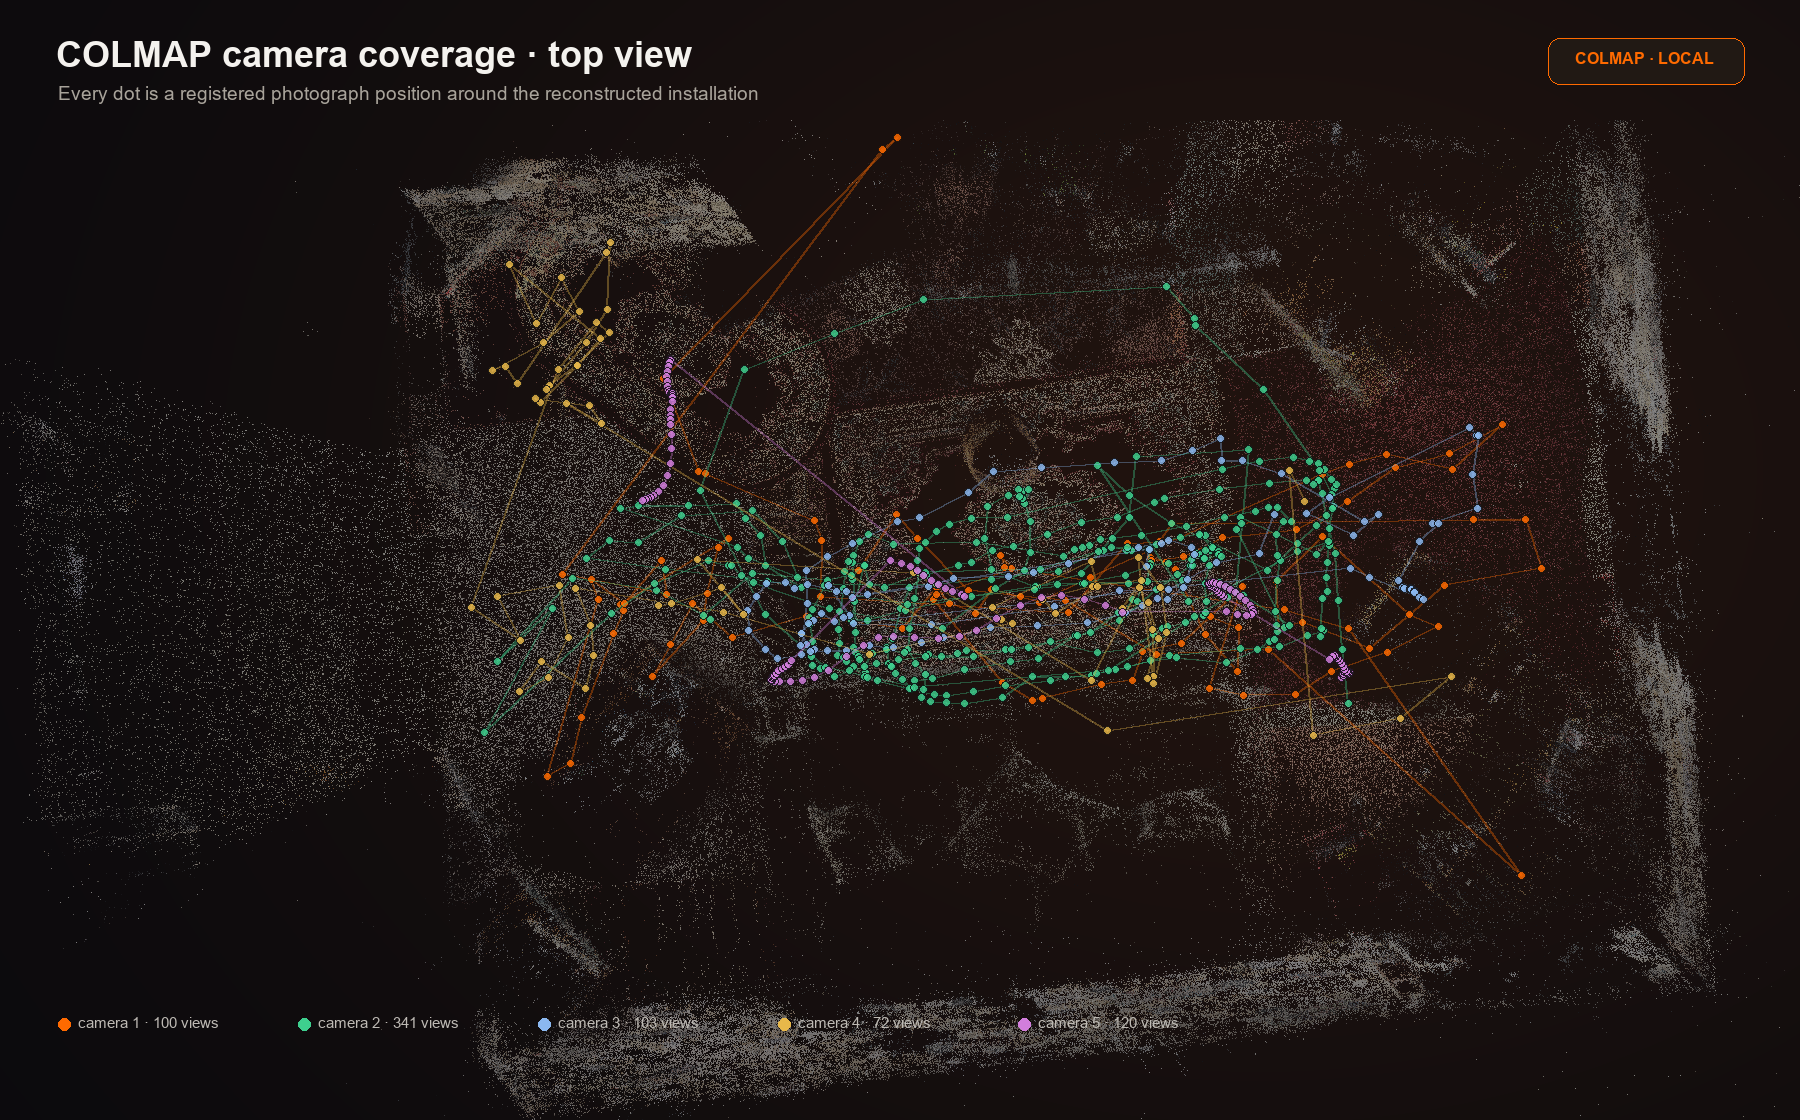
\includegraphics[width=0.96\columnwidth]{nested-cinema-colmap-camera-coverage.png}
\caption{COLMAP camera coverage over the room-set: the 222 registered stills and video frames
solved as two camera models. Source: UoS Vitrine repository (G. Watts).}
\label{fig:coverage}
\end{figure}


\subsection{Laptop and workstation measurements}
On the target laptop (RTX 3060 Laptop, \SI{6}{\giga\byte}) the validated run staged 222 images,
registered all of them, and recovered two camera models and 111{,}203 sparse points. Training
completed 15{,}000 iterations in \SI{60.4}{\minute}, ending at one million Gaussians with
full degree-three spherical harmonics, \SI{1.94}{\giga\byte} peak VRAM, and held-out metrics
of \SI{25.72}{\decibel} PSNR / 0.8167 SSIM. VRAM was never the binding constraint; elapsed
time was. The RTX 5090 control reused the proven recipe (768-pixel crop, 2048-pixel source,
one-million cap, 15k iterations) and reached \SI{25.06}{\decibel} / 0.8211 SSIM in
\SI{2.4}{\minute} at \SI{1.75}{\giga\byte}, matching laptop quality about 25 times faster.

Two measurements explain why time, not memory, binds the laptop. Rasterisation cost tracks
the number of Gaussians projected into the camera frustum, not the total population
(Table~\ref{tab:frustum}): an interior camera typically observes about a third of the room,
so the middle row is the practical basis for laptop estimates. The RTX 5090 reduces a
comparable step to 12--14\,ms, at which point kernel-launch overhead flattens the
frustum--time relationship. The same six profiles span both tiers by changing only measured
quantities (Table~\ref{tab:profiles}); the workstation-archive row records the investigated
configuration, not an approved preset.

\begin{table}[t]
\centering\small
\caption{Laptop frustum occupancy dominates iteration time (1.5M Gaussians, $768^2$, SH~3).
% SRC: report.md §4.1 (lines 193-199)
}
\label{tab:frustum}
\setlength{\tabcolsep}{5pt}
\begin{tabular}{@{}rr@{}}
\toprule
Gaussians in view & Time / iteration \\
\midrule
94\% & \SI{500}{\milli\second} \\
39\% & \SI{222}{\milli\second} \\
15\% & \SI{95}{\milli\second} \\
\bottomrule
\end{tabular}
\end{table}

\begin{table}[t]
\centering\small
\caption{Profiles. Same algorithm; only measured quantities change.
% SRC: report.md §4.3 (lines 209-214)
}
\label{tab:profiles}
\setlength{\tabcolsep}{3pt}
\begin{tabular}{@{}lrrrr@{}}
\toprule
Profile & Src & Crop & Cap & Iters \\
\midrule
laptop-draft       & 1600 & 512  & 400k & 7k \\
laptop-standard    & 2048 & 768  & 1.0M & 15k \\
laptop-archive     & 2560 & 768  & 1.5M & 30k \\
workstation-draft  & 2048 & 800  & 1.0M & 7k \\
workstation-standard & 3200 & 1280 & 3.0M & 20k \\
workstation-archive & 4096 & 1600 & 6.0M & 30k \\
\bottomrule
\end{tabular}
\end{table}

\subsection{Archive-profile opacity collapse}
Our strongest tested negative result isolates crop/source scale as the decisive variable
(Table~\ref{tab:collapse}). Both healthy runs use 768/2048; both collapsed runs use 1600/4096.
Reducing the cap from six million to one million did not restore the live population, and
correcting the position-learning-rate horizon did not either. In the large-crop runs the
fraction of Gaussians above the live-opacity threshold falls catastrophically: one random
1600-pixel crop from a 4096-pixel source does not revisit each Gaussian often enough for
reconstruction gradients to counter global opacity and scale regularisation, so MCMC relocates
dead splats from a shrinking live pool. The empirical conclusion that 1600/4096 is unsafe in the
current trainer is definitive; the mechanism remains a testable hypothesis. Live exported
population therefore belongs beside PSNR and SSIM --- a nominal six-million cap says little if
98.7\% of the population is effectively transparent.

\begin{table}[t]
\centering\small
\caption{RTX 5090 controlled matrix. Crop/source scale, not cap, tracks the collapse.
% SRC: report.md §5.3 table (lines 255-261)
}
\label{tab:collapse}
\setlength{\tabcolsep}{3pt}
\begin{tabular}{@{}lrrrr@{}}
\toprule
Run & Crop/src & Cap & Live g. & PSNR \\
\midrule
3060 baseline    & 768/2048  & 1.0M & 555k (55\%)  & 25.72 \\
5090 control     & 768/2048  & 1.0M & 528k (53\%)  & 25.06 \\
5090 candidate Q1& 1024/3072 & 1.5M & 940k (63\%)  & 24.71 \\
5090 safe-cap    & 1600/4096 & 1.0M & 2.2k (0.2\%) & 17.49 \\
5090 six-million & 1600/4096 & 6.0M & 80k (1.3\%)  & 14.31 \\
\bottomrule
\end{tabular}
\end{table}

A matched-view diagnostic on held-out still \texttt{IMG\_6351} (Figure~\ref{fig:photovsrecon}) shows both splat renders soften
sofa fabric, newspaper print and equipment detail that stay sharp in the source. The detail
exists in the stills but does not survive reconstruction; the indicated next test is a
stills-only baseline before reintroducing only the video frames that close a genuine coverage
gap. The 5090 control is the honest working workstation result: it reproduces laptop quality
about 25 times faster but does not yet exceed it.

\begin{figure*}[t]
\centering
% SRC: uos-vitrine/docs/images/nested-cinema-photo-vs-reconstruction.png (Glenn Watts, UoS Vitrine repo)
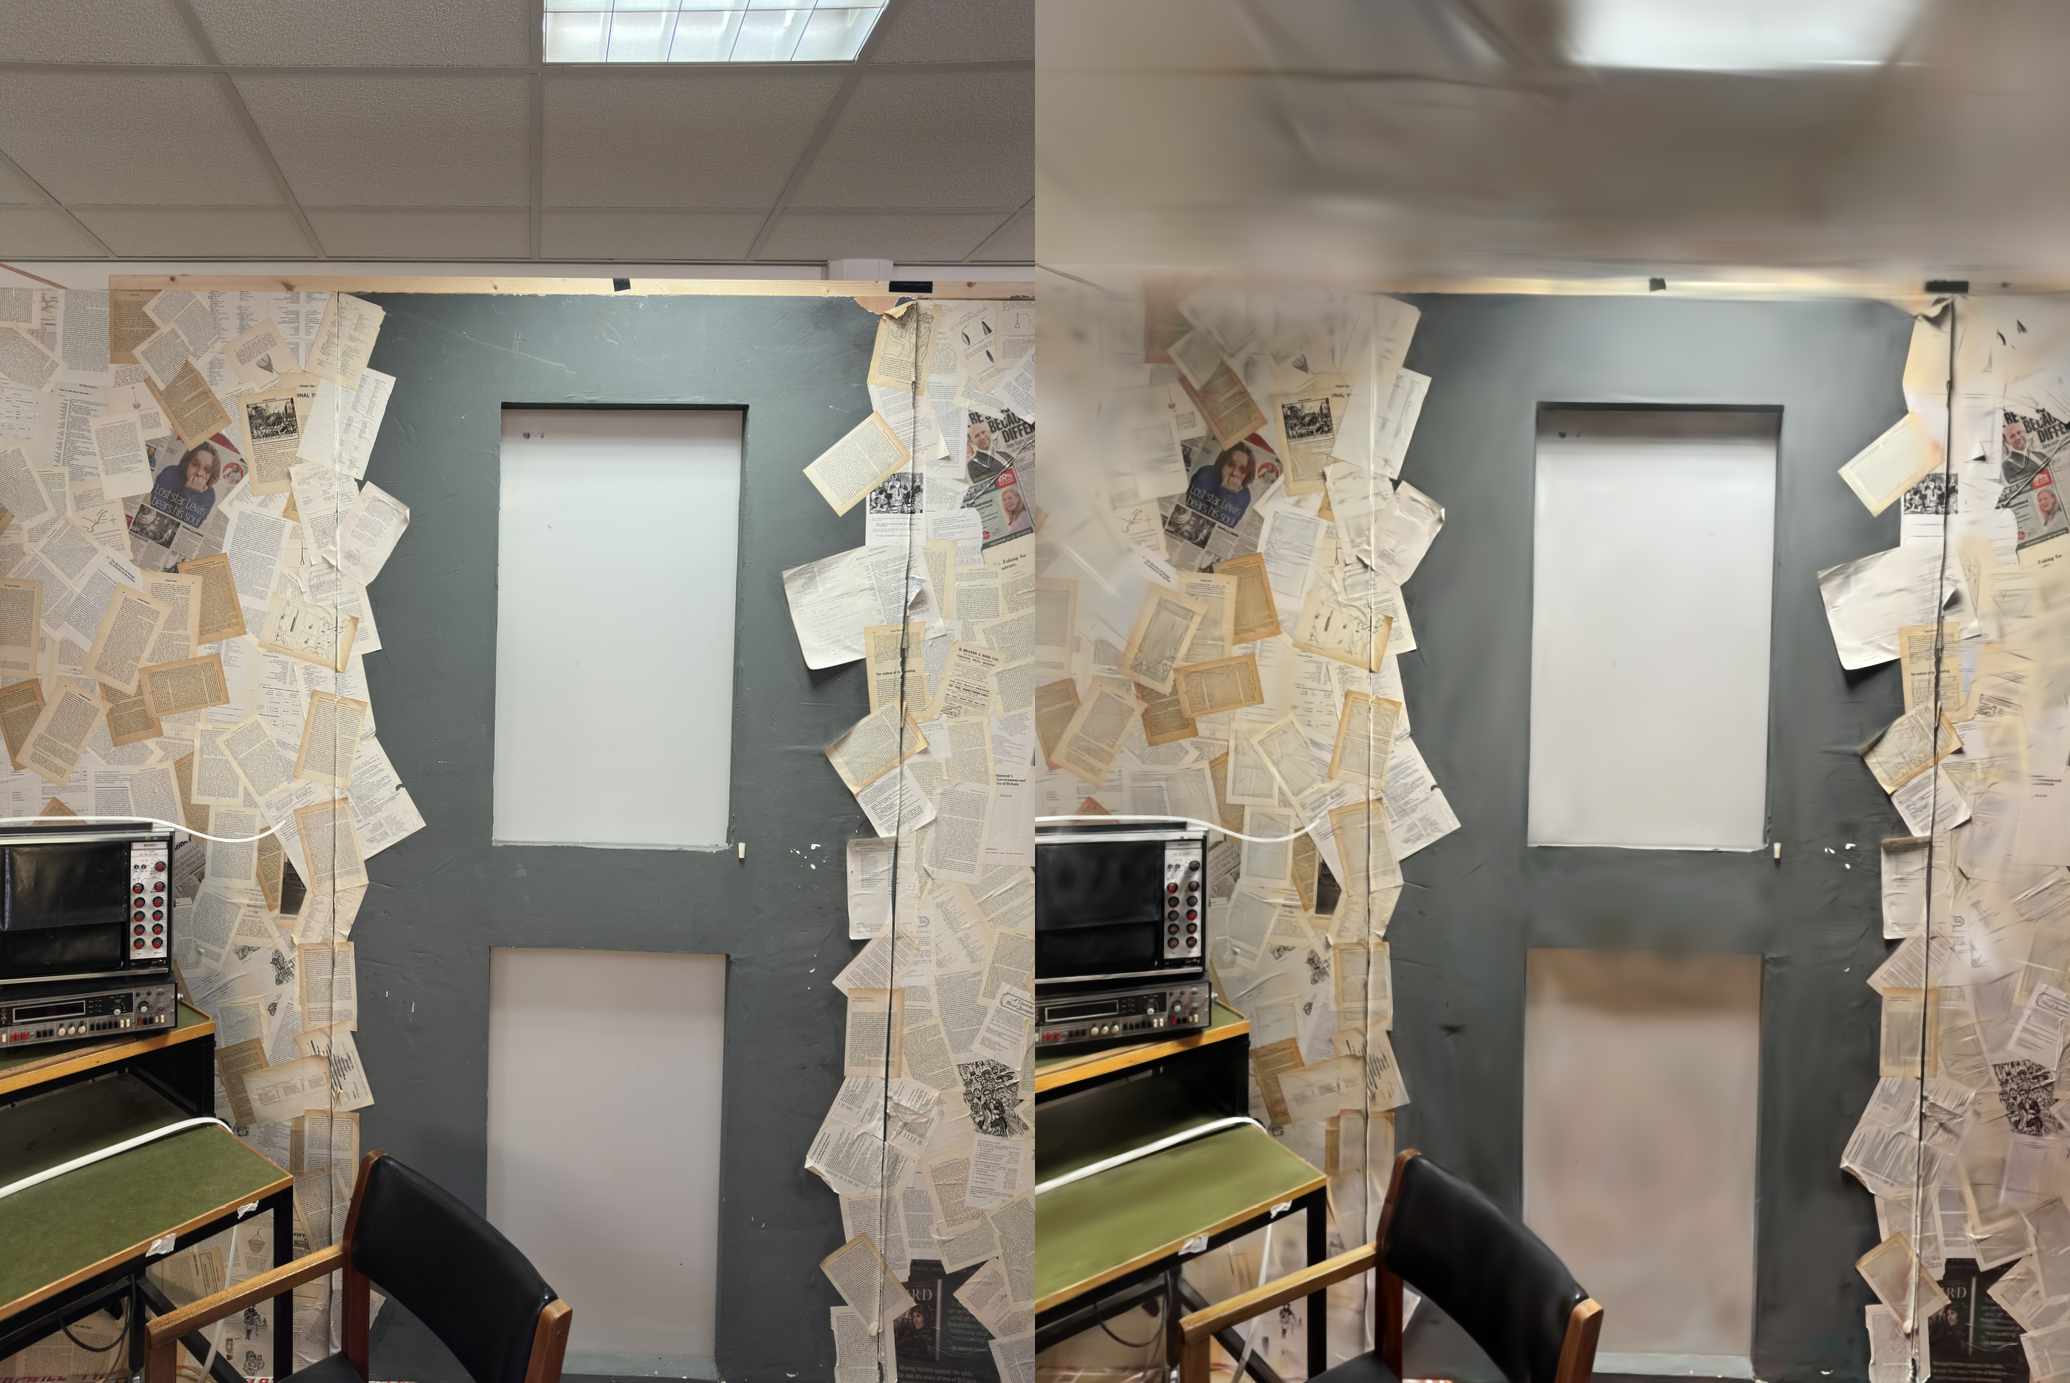
\includegraphics[width=0.92\textwidth]{nested-cinema-photo-vs-reconstruction.png}
\caption{Matched-view comparison on the newspaper partition: source photograph (left) against the
splat reconstruction (right) from the same COLMAP camera. The printed text and clip edges stay
sharp in the source and soften in the render --- the detail is present in the stills but does not
survive reconstruction. Source: UoS Vitrine repository (G. Watts).}
\label{fig:photovsrecon}
\end{figure*}


\subsection{Energy and cost}
The Windows runs sample GPU power through \texttt{nvidia-smi} and integrate it over training,
costed at the recorded \pounds0.2703/kWh tariff (Table~\ref{tab:energy}). The control trains for
about a third of a penny; the collapsed safe-cap run costs nearly four times as much to produce a
worse result. These figures cover sampled GPU power, not whole-system wall energy, so they are
valid for relative trainer comparison on this workstation but are not the full institutional cost.
A wall-socket meter is the preferred boundary for the planned sustainability integration.

\begin{table}[h]
\centering\small
\caption{Sampled-GPU energy and cost per 5090 run.
% SRC: report.md §5.3 energy table (lines 277-281)
}
\label{tab:energy}
\setlength{\tabcolsep}{4pt}
\begin{tabular}{@{}lrrl@{}}
\toprule
Run & Time & Energy & Cost \\
\midrule
Control 768/2048   & \SI{2.4}{\minute} & \SI{0.013}{kWh} & \pounds0.0035 \\
Q1 1024/3072       & \SI{3.0}{\minute} & \SI{0.018}{kWh} & \pounds0.0049 \\
Safe-cap 1600/4096 & \SI{7.6}{\minute} & \SI{0.049}{kWh} & \pounds0.0132 \\
\bottomrule
\end{tabular}
\end{table}

% SRC: DESIGN.md (stages 1-9); ADR-003; DDD-001; ADR-002
\section{Object pipeline: design and method}

It consumes a Vitrine run read-only and emits \texttt{objects/objects.json}
(schema \texttt{vitrine/object/1}) plus per-object GLBs and a composed scene. Nine stages
run under one evidence-vs-proposal discipline.

\textbf{Identify} runs GroundingDINO text prompts into SAM3.1 promptable segmentation per
frame, degrading to a fixed concept list rather than blocking. \textbf{Rectify} enforces an
explicit image-domain contract: the sidecar persists its own undistorted images and adjusted
intrinsics (because UoS never persists undistorted images), replicating \texttt{undistort.py}
maths under golden tests that require pixel-identical rectification for the same camera. Every
artefact records which pixel domain (distorted or rectified) it lives in.

\textbf{Carve} is the stage where correctness matters most. A 2D mask votes for 3D Gaussians only
through per-pixel front-depth-band gating (foreground / background / \emph{abstain}), with
min-view thresholds, 3D connected-component cleanup and robust p5--p95 extents. The naive
all-along-ray voting of the earlier DreamLab \texttt{mask\_projector} was rejected in adversarial
review because it labels occluded Gaussians behind the object; carve is golden-tested against the
gallery ground-truth object PLYs. \textbf{Seed} scores crops and views by silhouette area,
sharpness, centrality and edge clearance: Lane~A takes the single best matted crop, Lane~B the
top 8--16 diverse views. Splat renders are never used as conditioning.

\textbf{Generate} runs two lanes under one harness (\S\ref{sec:licence}). \textbf{Select}
renders every candidate from all recovered real cameras and scores silhouette IoU, masked
perceptual similarity, depth consistency on observed regions and mesh sanity, reporting observed
and withheld surfaces separately. \textbf{Place} is an owner hard requirement: it initialises
translation and scale from the carve centroid and extents, then refines full SE(3)+scale by
silhouette and photometric alignment against all real masks and frames. It is symmetry-aware and
fits scene-up (EXIF gravity, support-plane fit, or the LiDAR GLB cross-check on
nested-cinema-04) rather than assuming $+Y$. The composed scene rendered from real cameras is the
acceptance proof, and the manifest records per-axis observability, residuals and confidence.

\textbf{Finish} is the second hard requirement: UV unwrap (xatlas/Blender), then projective bake
of real rectified frames onto observed UV islands with per-texel best-view selection by angle,
sharpness and occlusion, and seam blending. Generative fill touches only unseen texels, recorded
in a per-texel provenance mask, followed by albedo delighting. Real frames constrain; generated
pixels propose, always flagged. \textbf{Manifest} writes one lineage record per object: sha256 of
every asset \emph{and} every checkpoint (repo, commit, hash, licence class), stage scores, coverage
estimate, orientation observability and VRAM peaks. No stage may silently substitute generated data
where evidence exists; a missing stage output degrades the record's status field, never fakes it.

\begin{figure}[h]
\centering
% SRC: seed crops runs/nc04-object-pass1/seed/ + Blender renders of runs/nc04-generate-pass1/*/ (scripts/render_turntable.py)
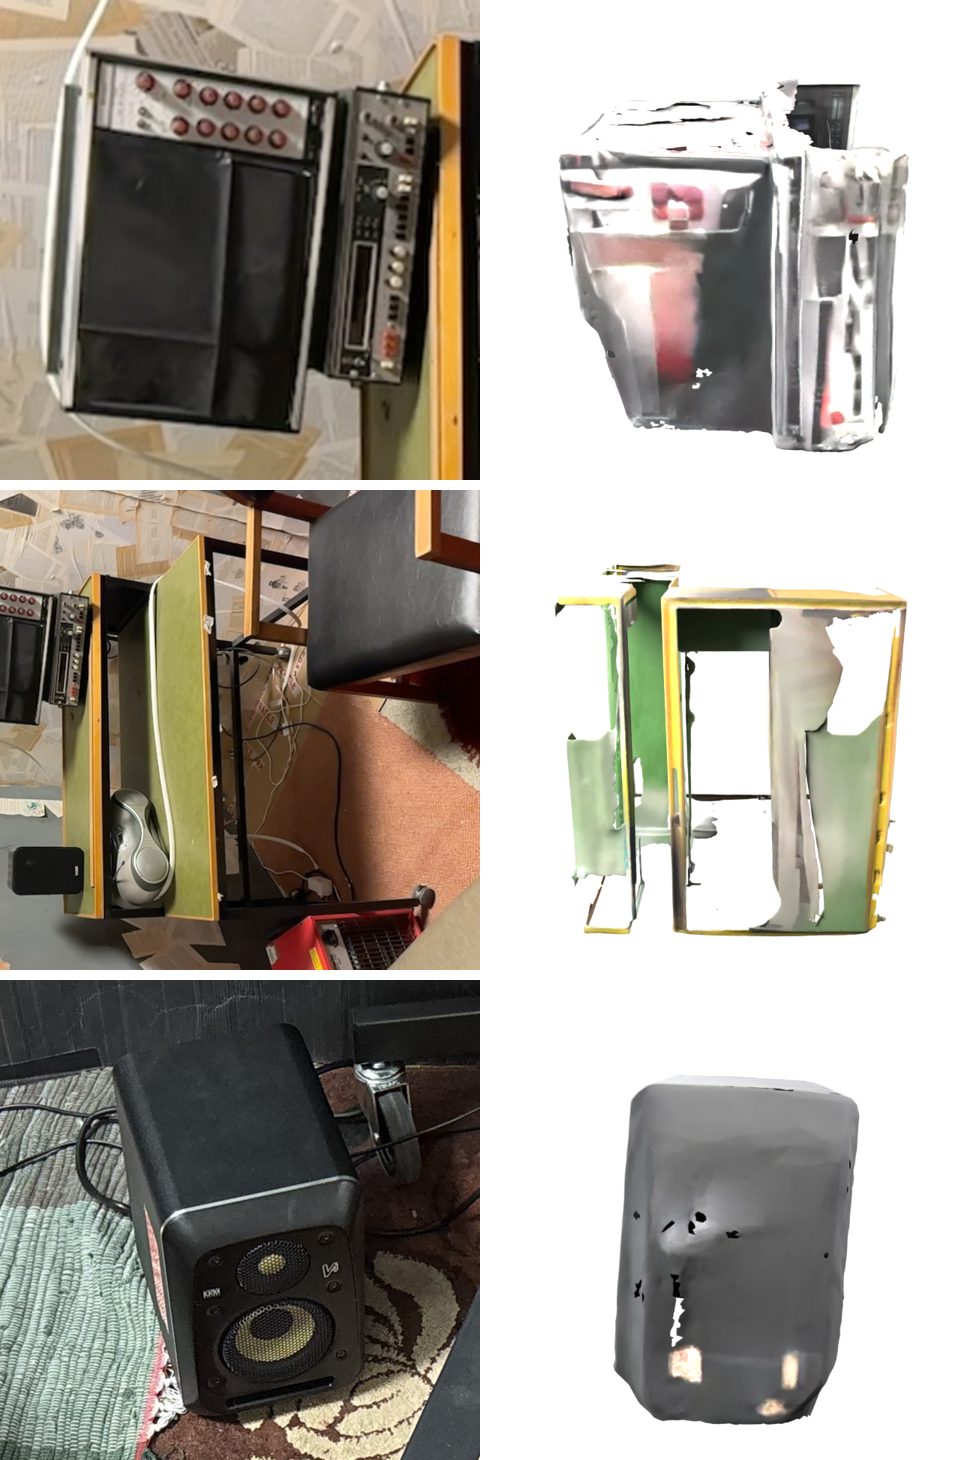
\includegraphics[width=0.86\columnwidth]{renders/assets_pairs.png}
\caption{From one photograph to an asset: the evidence-scored seed crop (left) and the Lane-A
TRELLIS.2 reconstruction rendered from a fresh view (right), for radio, table and speaker. The
generated geometry carries the crop's colour and structure; unobserved faces are inferred.}
\label{fig:assetpairs}
\end{figure}

% SRC: nc04-object-pass1/REPORT.md (all numbers, camera table, object table)
\section{Live results: Nested Cinema 04}

Run \texttt{nc04-object-pass1} was the sidecar's first contact with the real scene, on an
RTX 6000 Ada, wall-time \SI{352}{\second}. The COLMAP model holds 736 registered images
across five OPENCV cameras and a 2.0M-Gaussian splat; 79 frames were selected by stratified
sampling. Camera~5, a 4K walkthrough of 120 registered frames, contributes nothing because
the package ships only the \texttt{.MOV} and no frames were extracted; video decode is out of
scope for pass~1, so this is recorded as an explicit gap. Rectify dominated wall-time
(\SI{227}{\second} of \SI{352}{\second}) through HEIC decode and full-resolution undistort of the
3200-class frames.

Six object candidates were carved (Table~\ref{tab:nc04}). Four are well-supported: the table
(most-supported, 21 views), the vintage radio, and two speakers that \texttt{carve\_components}
correctly separated as distinct 3D instances from one \texttt{speaker} mask set. Two are
problematic: \texttt{armchair chair} rests on only two views (a confidence of 1.00 is unreliable
at that count, and the label is phrase-merged), and \texttt{radio\#1} is a smaller second component
that may be a genuine second unit or a fragment. Seed crops confirm real installation objects: vintage
radios, cassette decks, a record-player case, a table. Figure~\ref{fig:seedcrops} shows
three of the evidence-scored seed crops.

\begin{table}[t]
\centering\small
\caption{nc04 object candidates. Four well-carved, two marginal.
% SRC: nc04-object-pass1/REPORT.md object table (lines 22-30)
}
\label{tab:nc04}
\setlength{\tabcolsep}{4pt}
\begin{tabular}{@{}lrrcl@{}}
\toprule
Label & Gauss. & conf & views & verdict \\
\midrule
table          & 38{,}383 & 0.80 & 21 & good (best) \\
radio \#0      & 17{,}276 & 0.87 & 16 & good \\
armchair chair & 19{,}055 & 1.00 & 2  & weak \\
speaker \#0    & 6{,}754  & 0.80 & 15 & good \\
speaker \#1    & 3{,}202  & 0.95 & 15 & good (2nd inst.) \\
radio \#1      & 6{,}286  & 0.87 & 16 & fair (fragment?) \\
\bottomrule
\end{tabular}
\end{table}

\begin{figure}[t]
\centering
\begin{subfigure}{0.31\columnwidth}
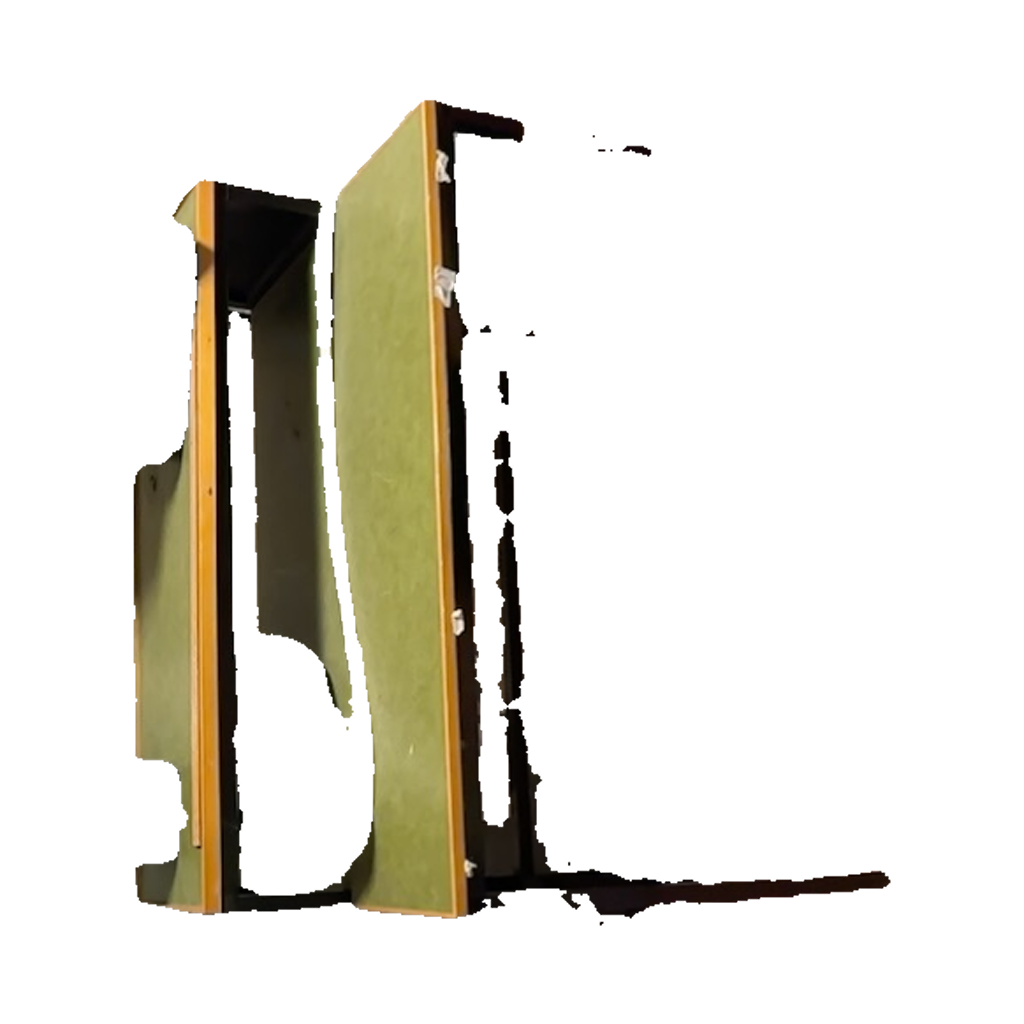
\includegraphics[width=\linewidth]{nc04-object-pass1/seed/table_00_crop.png}
\caption*{\tiny table}
\end{subfigure}\hfill
\begin{subfigure}{0.31\columnwidth}
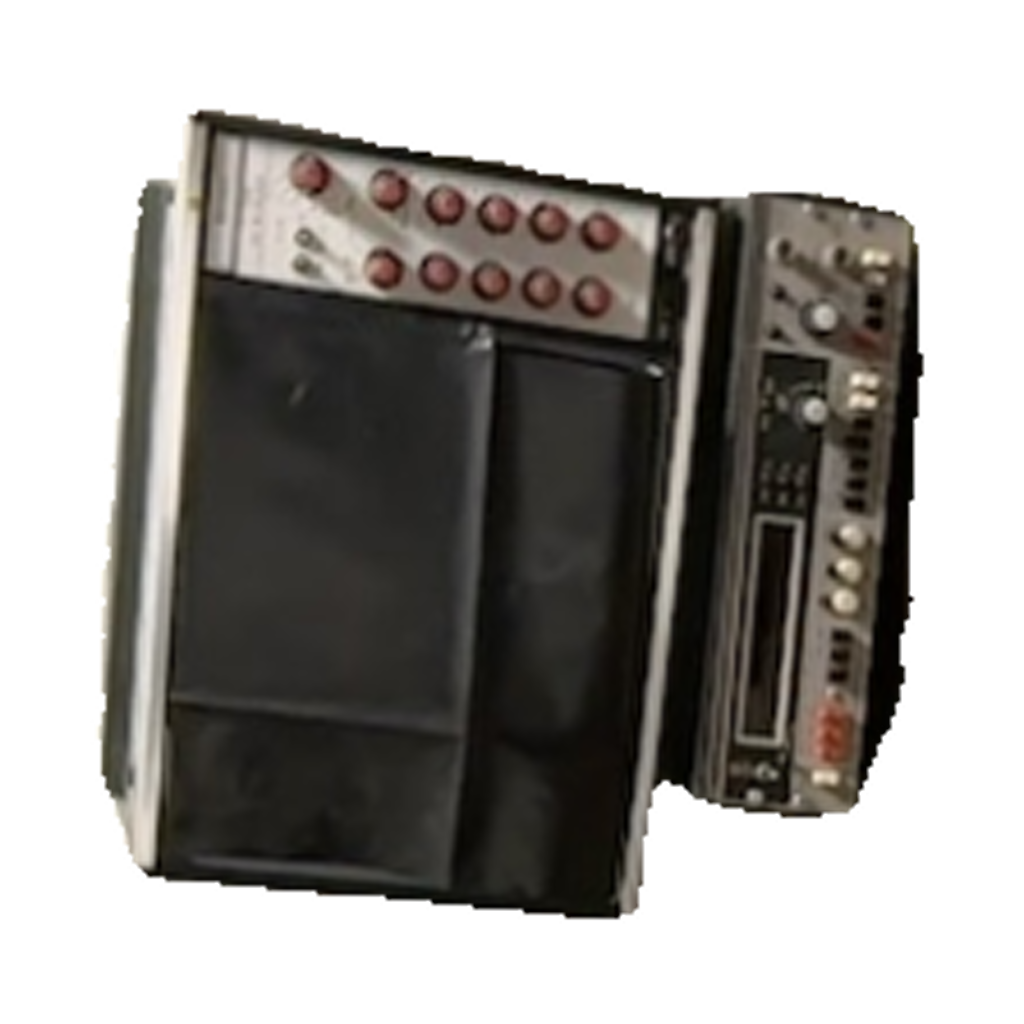
\includegraphics[width=\linewidth]{nc04-object-pass1/seed/radio_00_crop.png}
\caption*{\tiny radio}
\end{subfigure}\hfill
\begin{subfigure}{0.31\columnwidth}
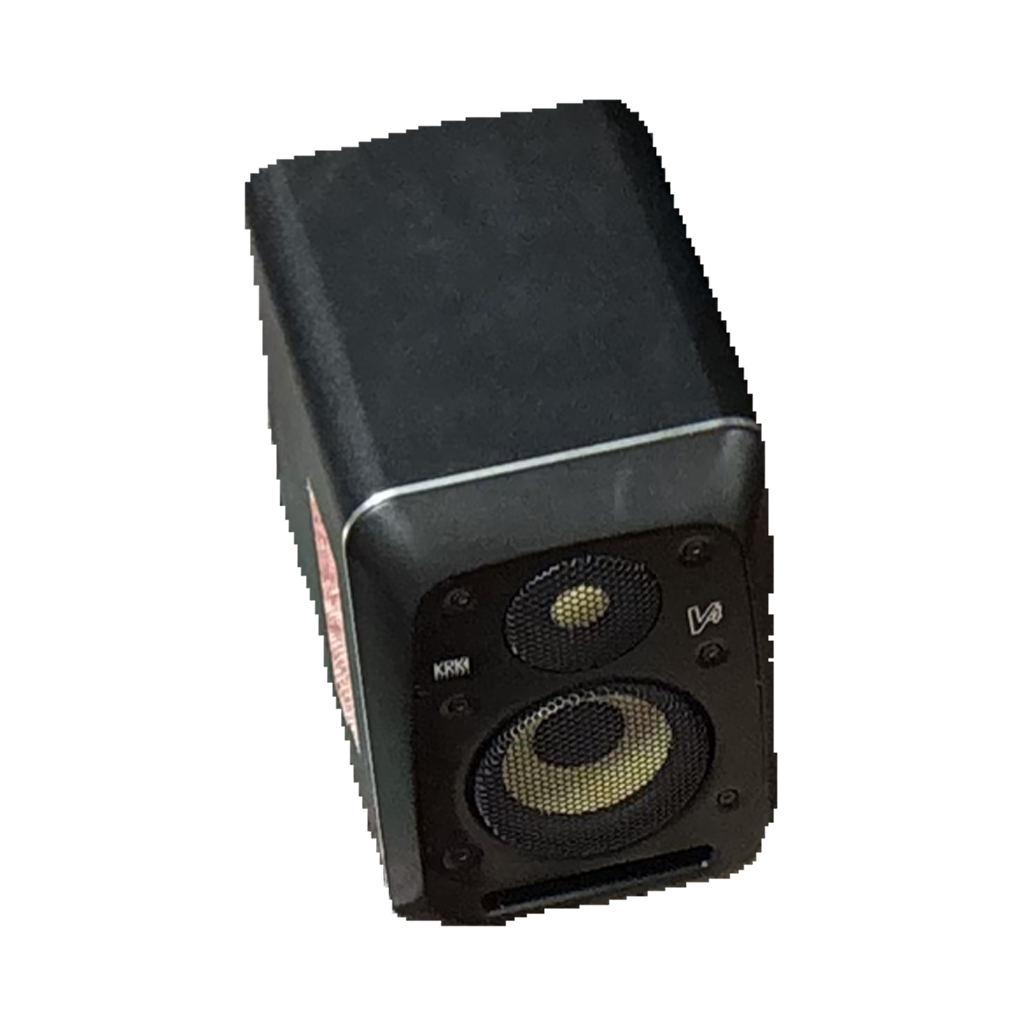
\includegraphics[width=\linewidth]{nc04-object-pass1/seed/speaker_00_crop.png}
\caption*{\tiny speaker}
\end{subfigure}
\caption{Evidence-scored seed crops from the live installation.
% SRC: runs/nc04-object-pass1/seed/*.png
}
\label{fig:seedcrops}
\end{figure}

\begin{figure}[t]
\centering
% SRC: runs/nc04-object-pass1/summary.json via scripts/make_closeout_charts.py
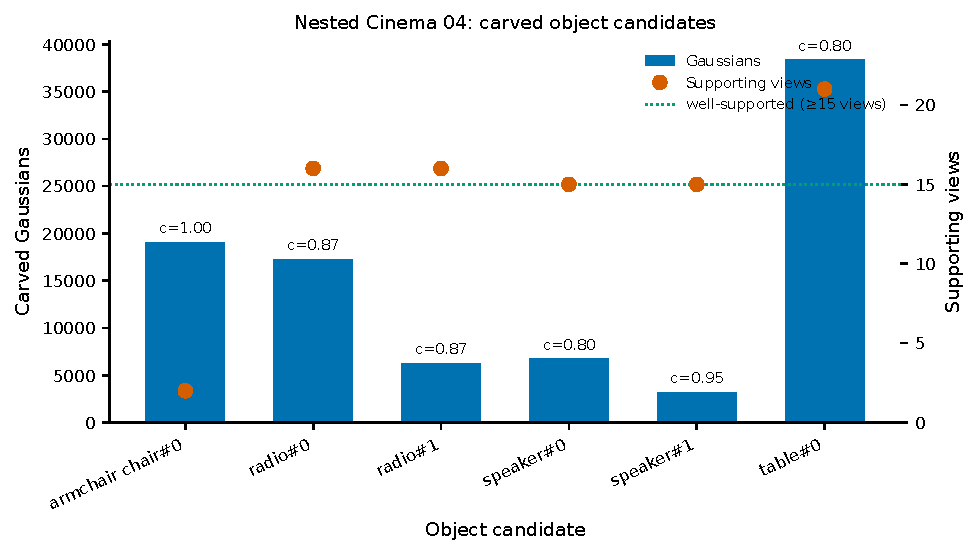
\includegraphics[width=\columnwidth]{nc04-object-pass1/charts/nc04_objects.pdf}
\caption{Carved candidates: Gaussian count (bars), supporting views (markers) and carve
confidence. The two below the 15-view line (armchair at 2 views, radio\#1 fragment) are the
weak pair.}
\label{fig:nc04objects}
\end{figure}

\subsection{Carve metrics on the golden set}
On the gallery golden set the full object path ran over 121 frames and scored each carved object
against 33 ground-truth object clouds. Every eval metric computes --- the primary validation goal.
Carve localises the right region but does not yet separate instances on an adversarial scene: the
gallery is wall-to-wall same-class paintings, so per-label mask unions cover most of each frame and
carve votes a large fraction of the splat foreground. Three ``objects'' of 1.5--2.4M Gaussians each
overlap ground-truth \texttt{object\_035} with high reproj-IoU (0.84--0.89) but only 3D-F1 $\approx$
0.35; smaller 3D components recover individual objects better (best 3D-F1 0.519) but many are
fragments (F1 $<$ 0.15). This contrasts with nested-cinema-04, where discrete, spatially separated
objects carved cleanly. The method is sound where objects are separated and degrades where a class
tiles the scene; per-instance masks rather than per-label unions are the primary fix.

\subsection{Per-instance carve: pass 1 to pass 2}
% SRC: runs/nc04-object-pass2/summary.json (frames, objects, rejected, timings)
Pass~2 selected all 736 registered frames (including Camera~5's walkthrough, now extracted) and
switched carve to per-instance masks. Object support rose sharply: \texttt{radio\#0} went from
17{,}276 Gaussians over 16 views to 118{,}070 over 331, \texttt{table\#0} to 39{,}155 over 250,
\texttt{speaker\#0} to 52{,}964 over 242. Nine candidates passed and three were rejected on the
min-view floor (\texttt{armchair}, \texttt{gramophone}, \texttt{mirror}, all
\texttt{insufficient\_views}) rather than kept as weak detections --- the pass-1 ``weak pair''
problem is now handled by a rejected list, not a caveat. The cost is wall-time: full-frame rectify
and identify push the pass to \SI{4662}{\second}, dominated by rectify (\SI{2297}{\second}) and
identify (\SI{1891}{\second}).

\subsection{Generation bake-off}\label{sec:objgen}
% SRC: runs/nc04-generate-pass1/*/candidates.json (Lane A); models-lane2/STATUS.md §Lane-B
Both lanes produced assets whose reserved VRAM was measured under Linux/Ada below the 32\,GB target
(Figure~\ref{fig:bakeoff}, \S\ref{sec:licence}); the Windows 11 / RTX 5090 acceptance run is still required.
\textbf{Lane~A} (TRELLIS.2, single matted crop at $1024^3$) generated 12 of 12 candidates ---
radio, table and speaker $\times$ four seeds --- with no failures. Reserved-VRAM peaks were
\SI{9.1}{\giga\byte} (radio), \SI{5.3}{\giga\byte} (table) and \SI{7.7}{\giga\byte} (speaker),
and per-seed runtimes ran \SIrange{37}{120}{\second}. \textbf{Lane~B} (ReconViaGen, textured GLB)
produced a single-view radio at \SI{15.0}{\giga\byte} and a multi-view radio (top-8 IoU-ranked
views) at \SI{16.6}{\giga\byte}; both textured GLBs are $\approx$17\,MB. Every variant stayed under 32\,GB reserved on the 48\,GB Ada
dev card, Lane~A with roughly $3.5\times$ headroom --- Linux/Ada evidence, not a Blackwell/5090 result.

A first \texttt{composed\_scene.glb} exists for the radio, placing the Lane-A and Lane-B assets
into the scene at solved transforms under an explicit basis contract (Figure~\ref{fig:composed}). Each object carries
provenance classes in \texttt{composed\_scene\_objects.json}: \texttt{geometry\_class=generated},
\texttt{material\_class=generated}, \texttt{placement\_class=carve-init}, and
\texttt{derivative\_class=composed-derivative}, so the placement is marked as carve-centroid
initialised, not yet silhouette-refined.

\begin{figure*}[t]
\centering
% SRC: runs/nc04-generate-pass1/radio/composed_proof/*.png (sidecar compose stage, real nc04 cameras)
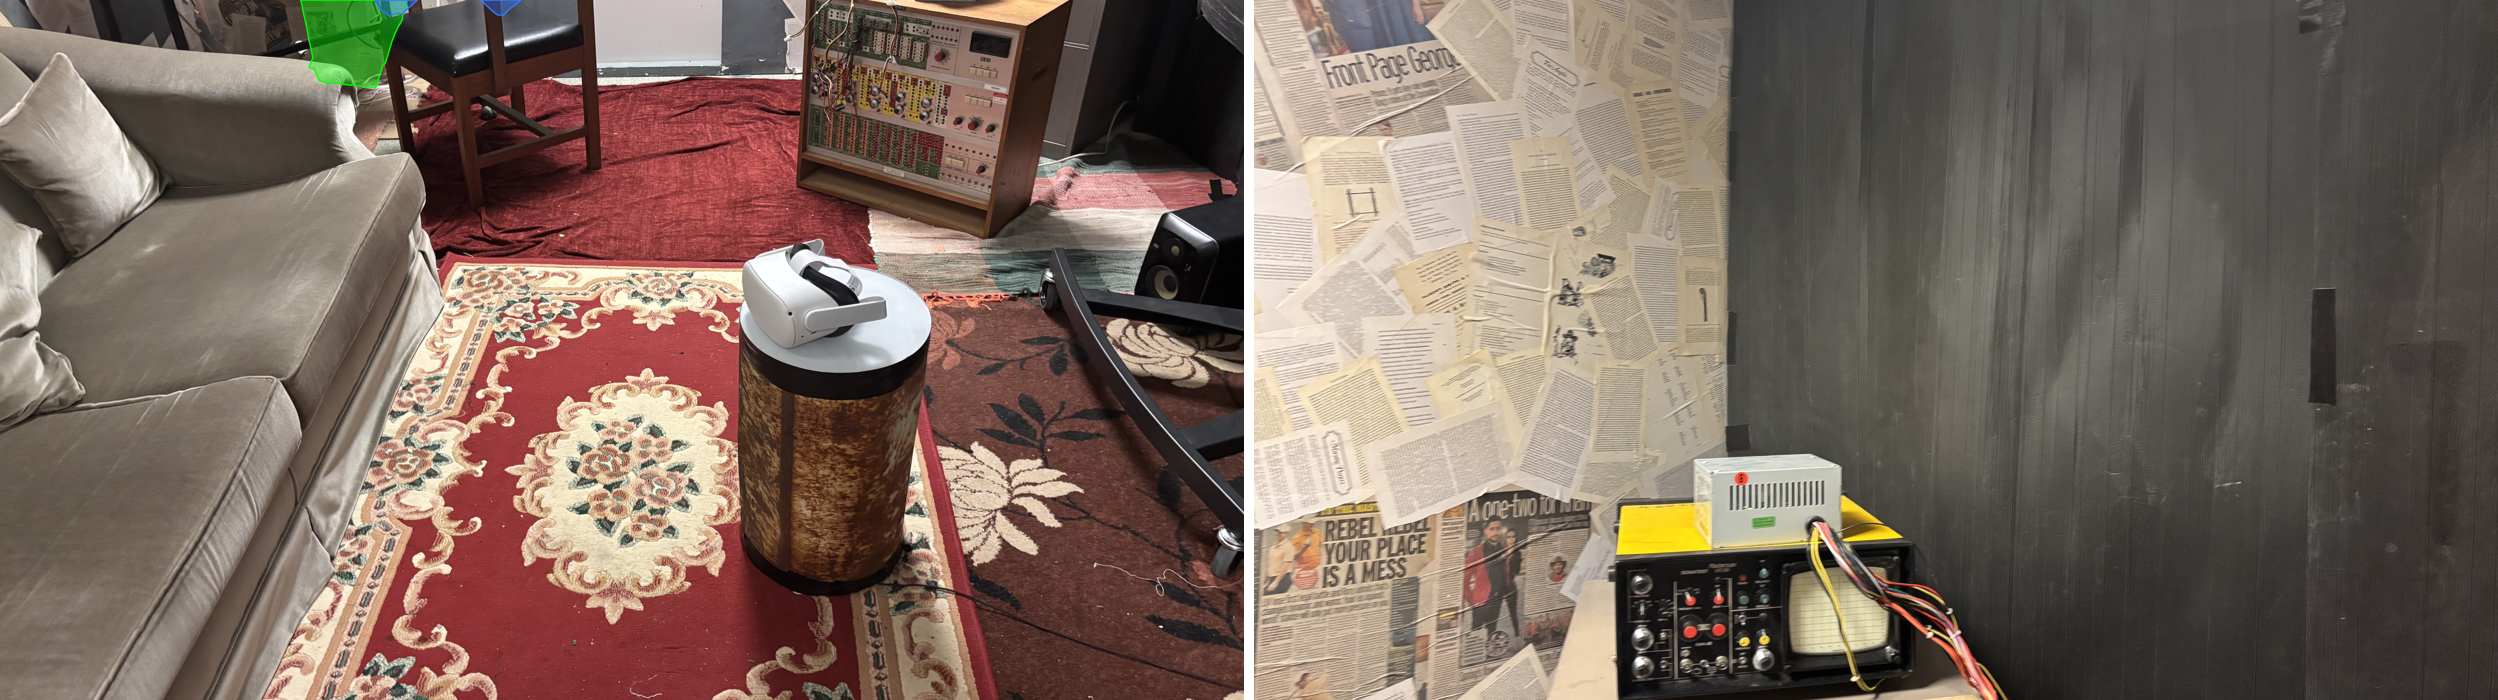
\includegraphics[width=0.98\textwidth]{renders/composed_proof.png}
\caption{Composed-scene proof: the generated radio placed back into the real Nested Cinema 04
room and rendered from two real COLMAP cameras. Green is the Lane-A (TRELLIS.2) silhouette, blue the
Lane-B (ReconViaGen) silhouette, composited over the real rectified frame at the solved placement.
Placement is evidence-based but carve-centroid initialised (\texttt{placement\_class=carve-init}, yaw
unrefined), so the overlay is roughly rather than precisely registered --- see the carve-contamination
note in \S\ref{sec:eval-ranking}.}
\label{fig:composed}
\end{figure*}

\begin{figure}[h]
\centering
% SRC: runs/nc04-generate-pass1/*/candidates.json + models-lane2/STATUS.md via make_closeout_charts.py
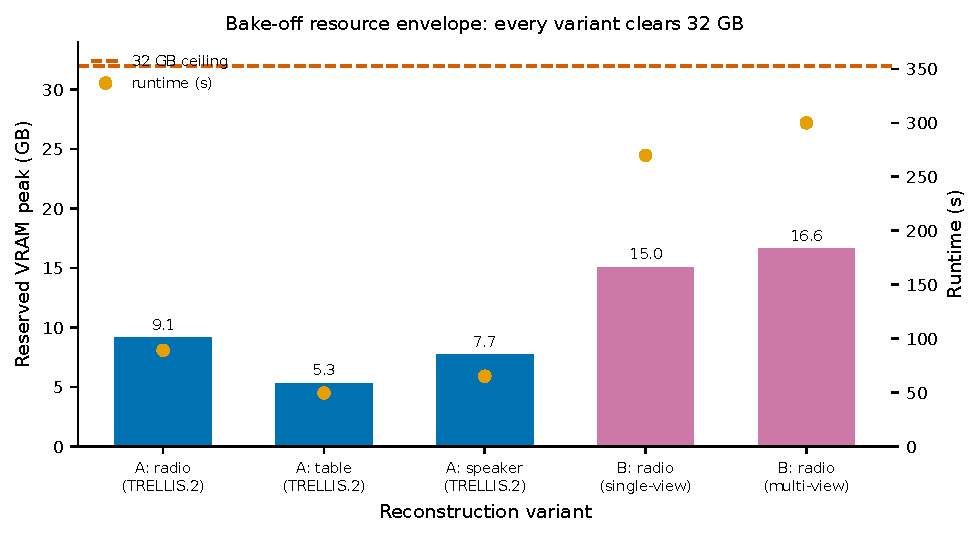
\includegraphics[width=\columnwidth]{nc04-generate-pass1/charts/bakeoff_vram.pdf}
\caption{Bake-off resource envelope: reserved-VRAM peak per variant against the 32\,GB ceiling,
with runtime. Lane-A peaks are the max across four seeds; Lane-B are the textured single/multi-view
runs.}
\label{fig:bakeoff}
\end{figure}

\begin{figure}[h]
\centering
% SRC: Blender turntables of runs/nc04-generate-pass1/{radio,table,speaker} best seeds (scripts/render_turntable.py)
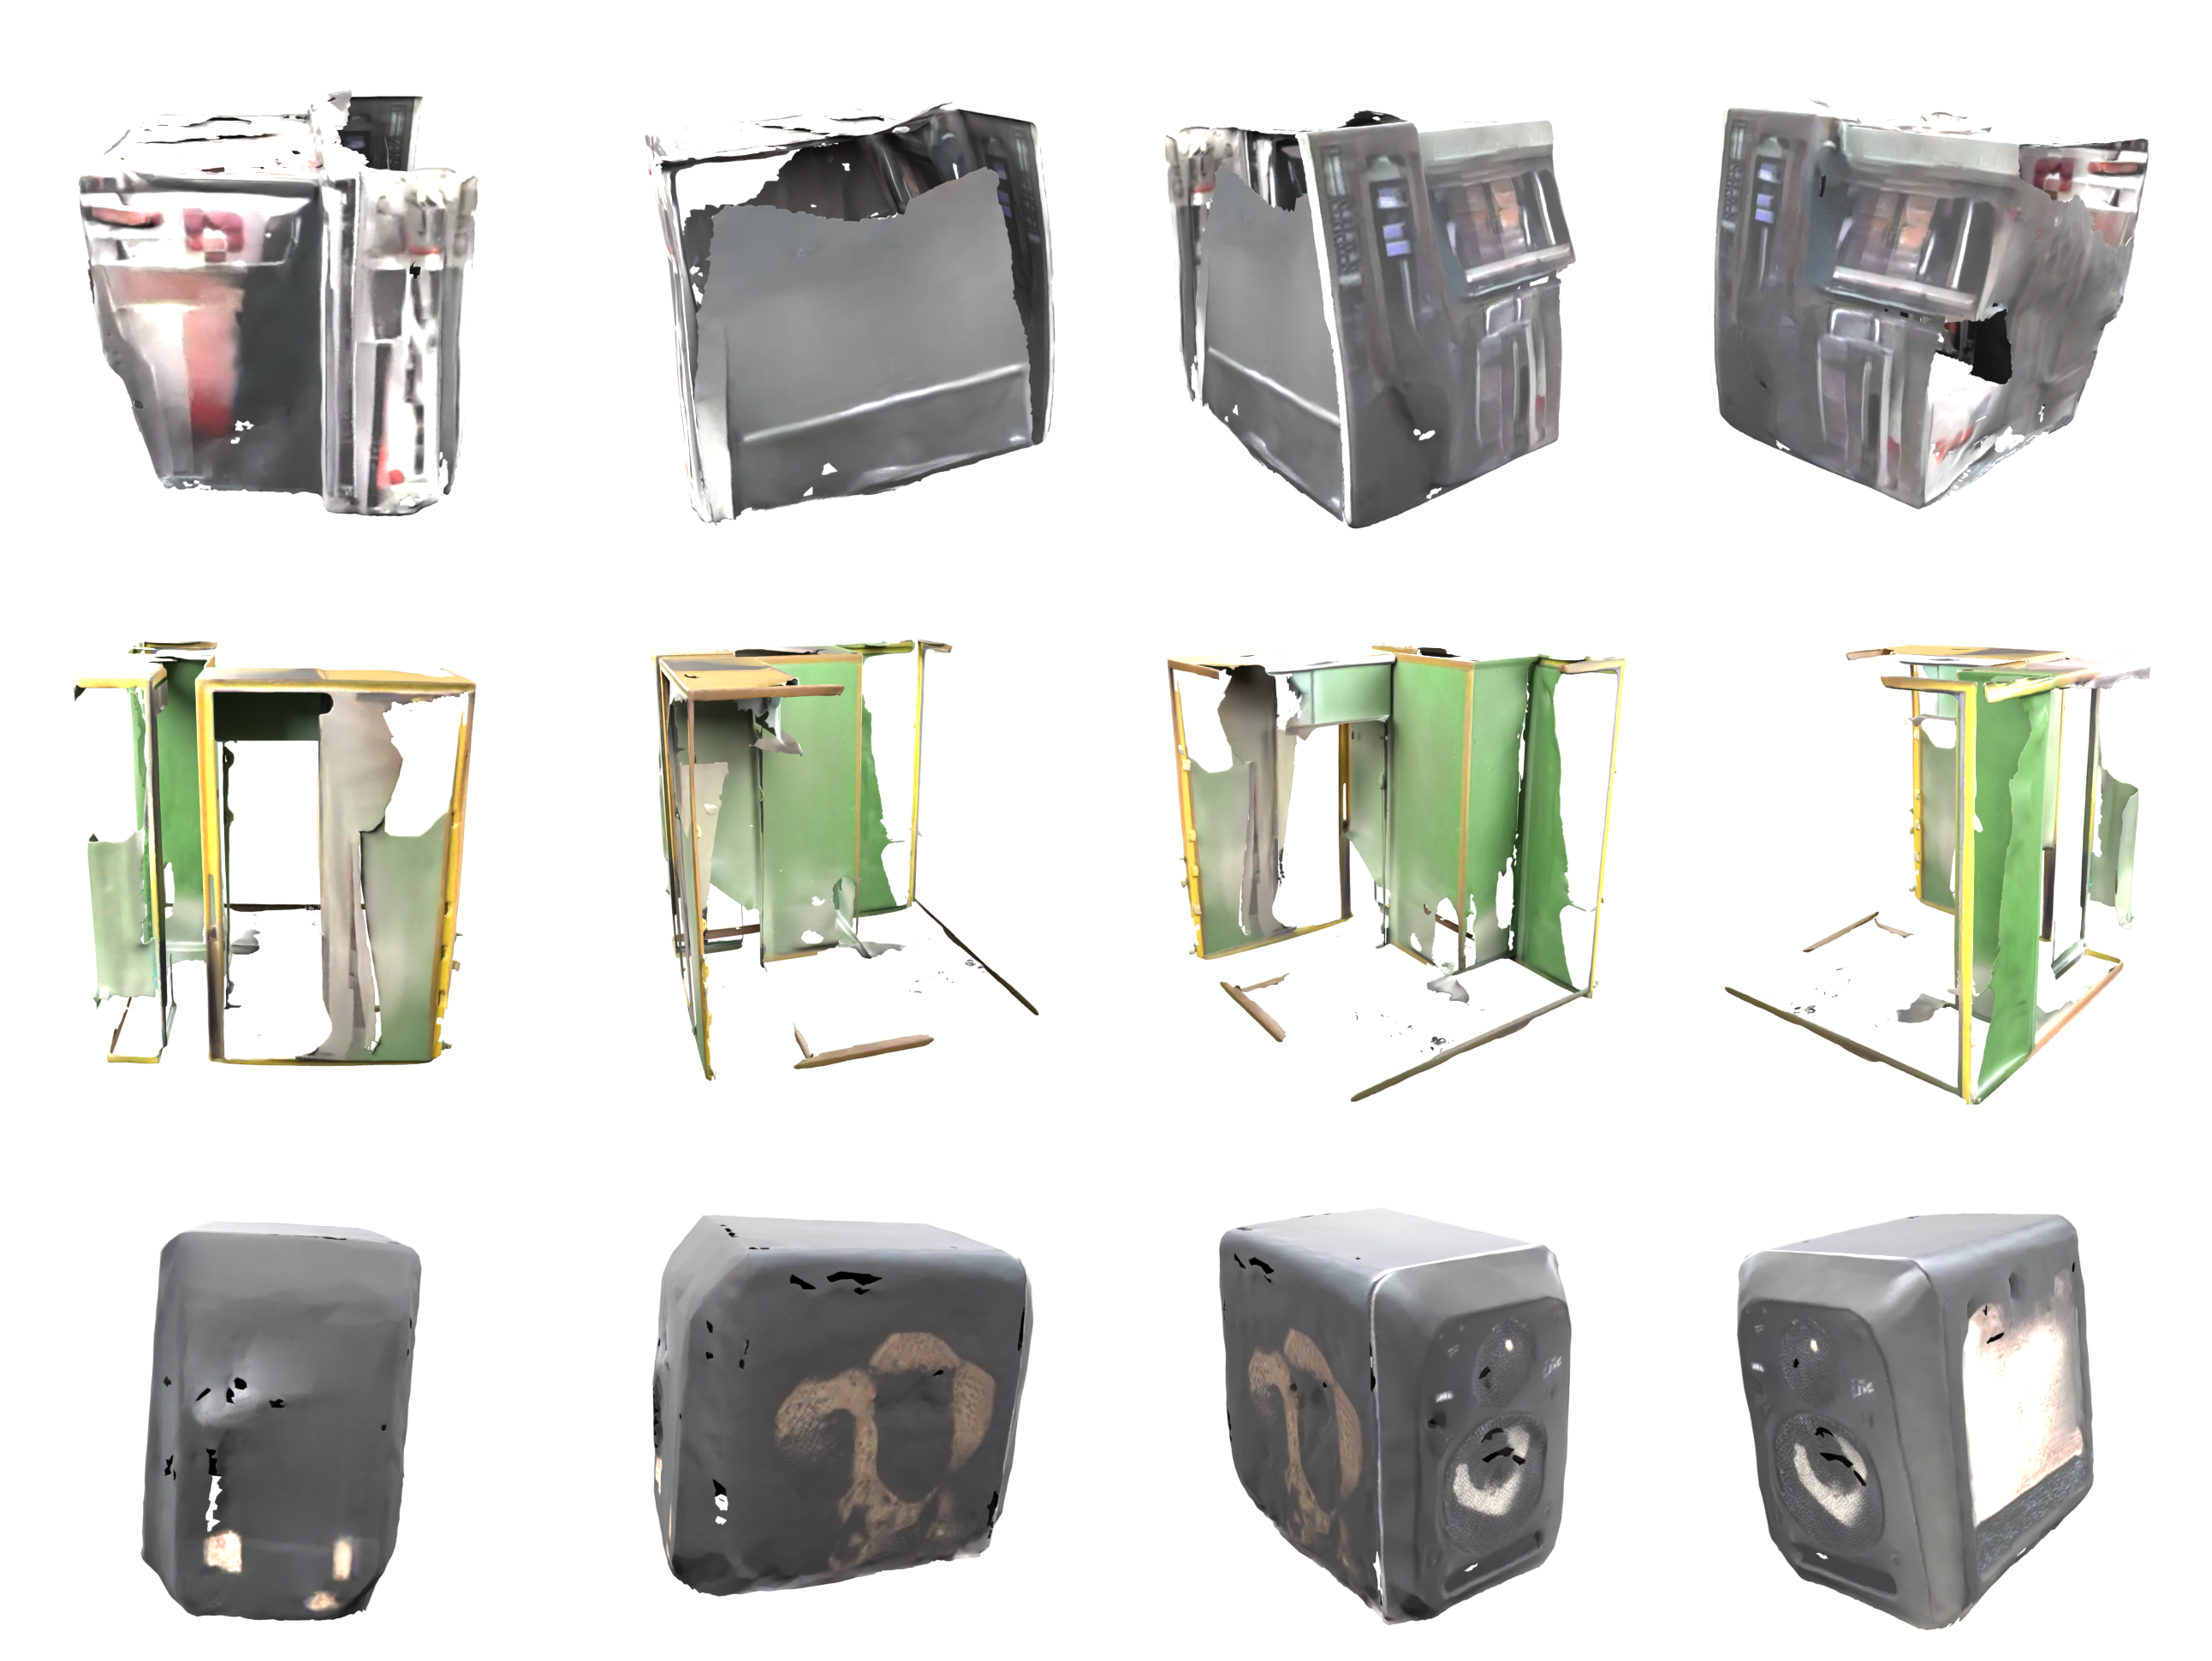
\includegraphics[width=\columnwidth]{renders/laneA_turntables.png}
\caption{Lane-A TRELLIS.2 objects, four turntable views each (radio, table, speaker; best seed by
mesh detail). Real generated 3D assets with baked texture; carving and single-crop generation leave
visible holes on unobserved backs.}
\label{fig:turntables}
\end{figure}

\begin{figure*}[t]
\centering
% SRC: Blender turntables, runs/nc04-generate-pass1/radio (Lane A) vs runs/nc04-laneb-pass1/radio_00_multiview (Lane B)
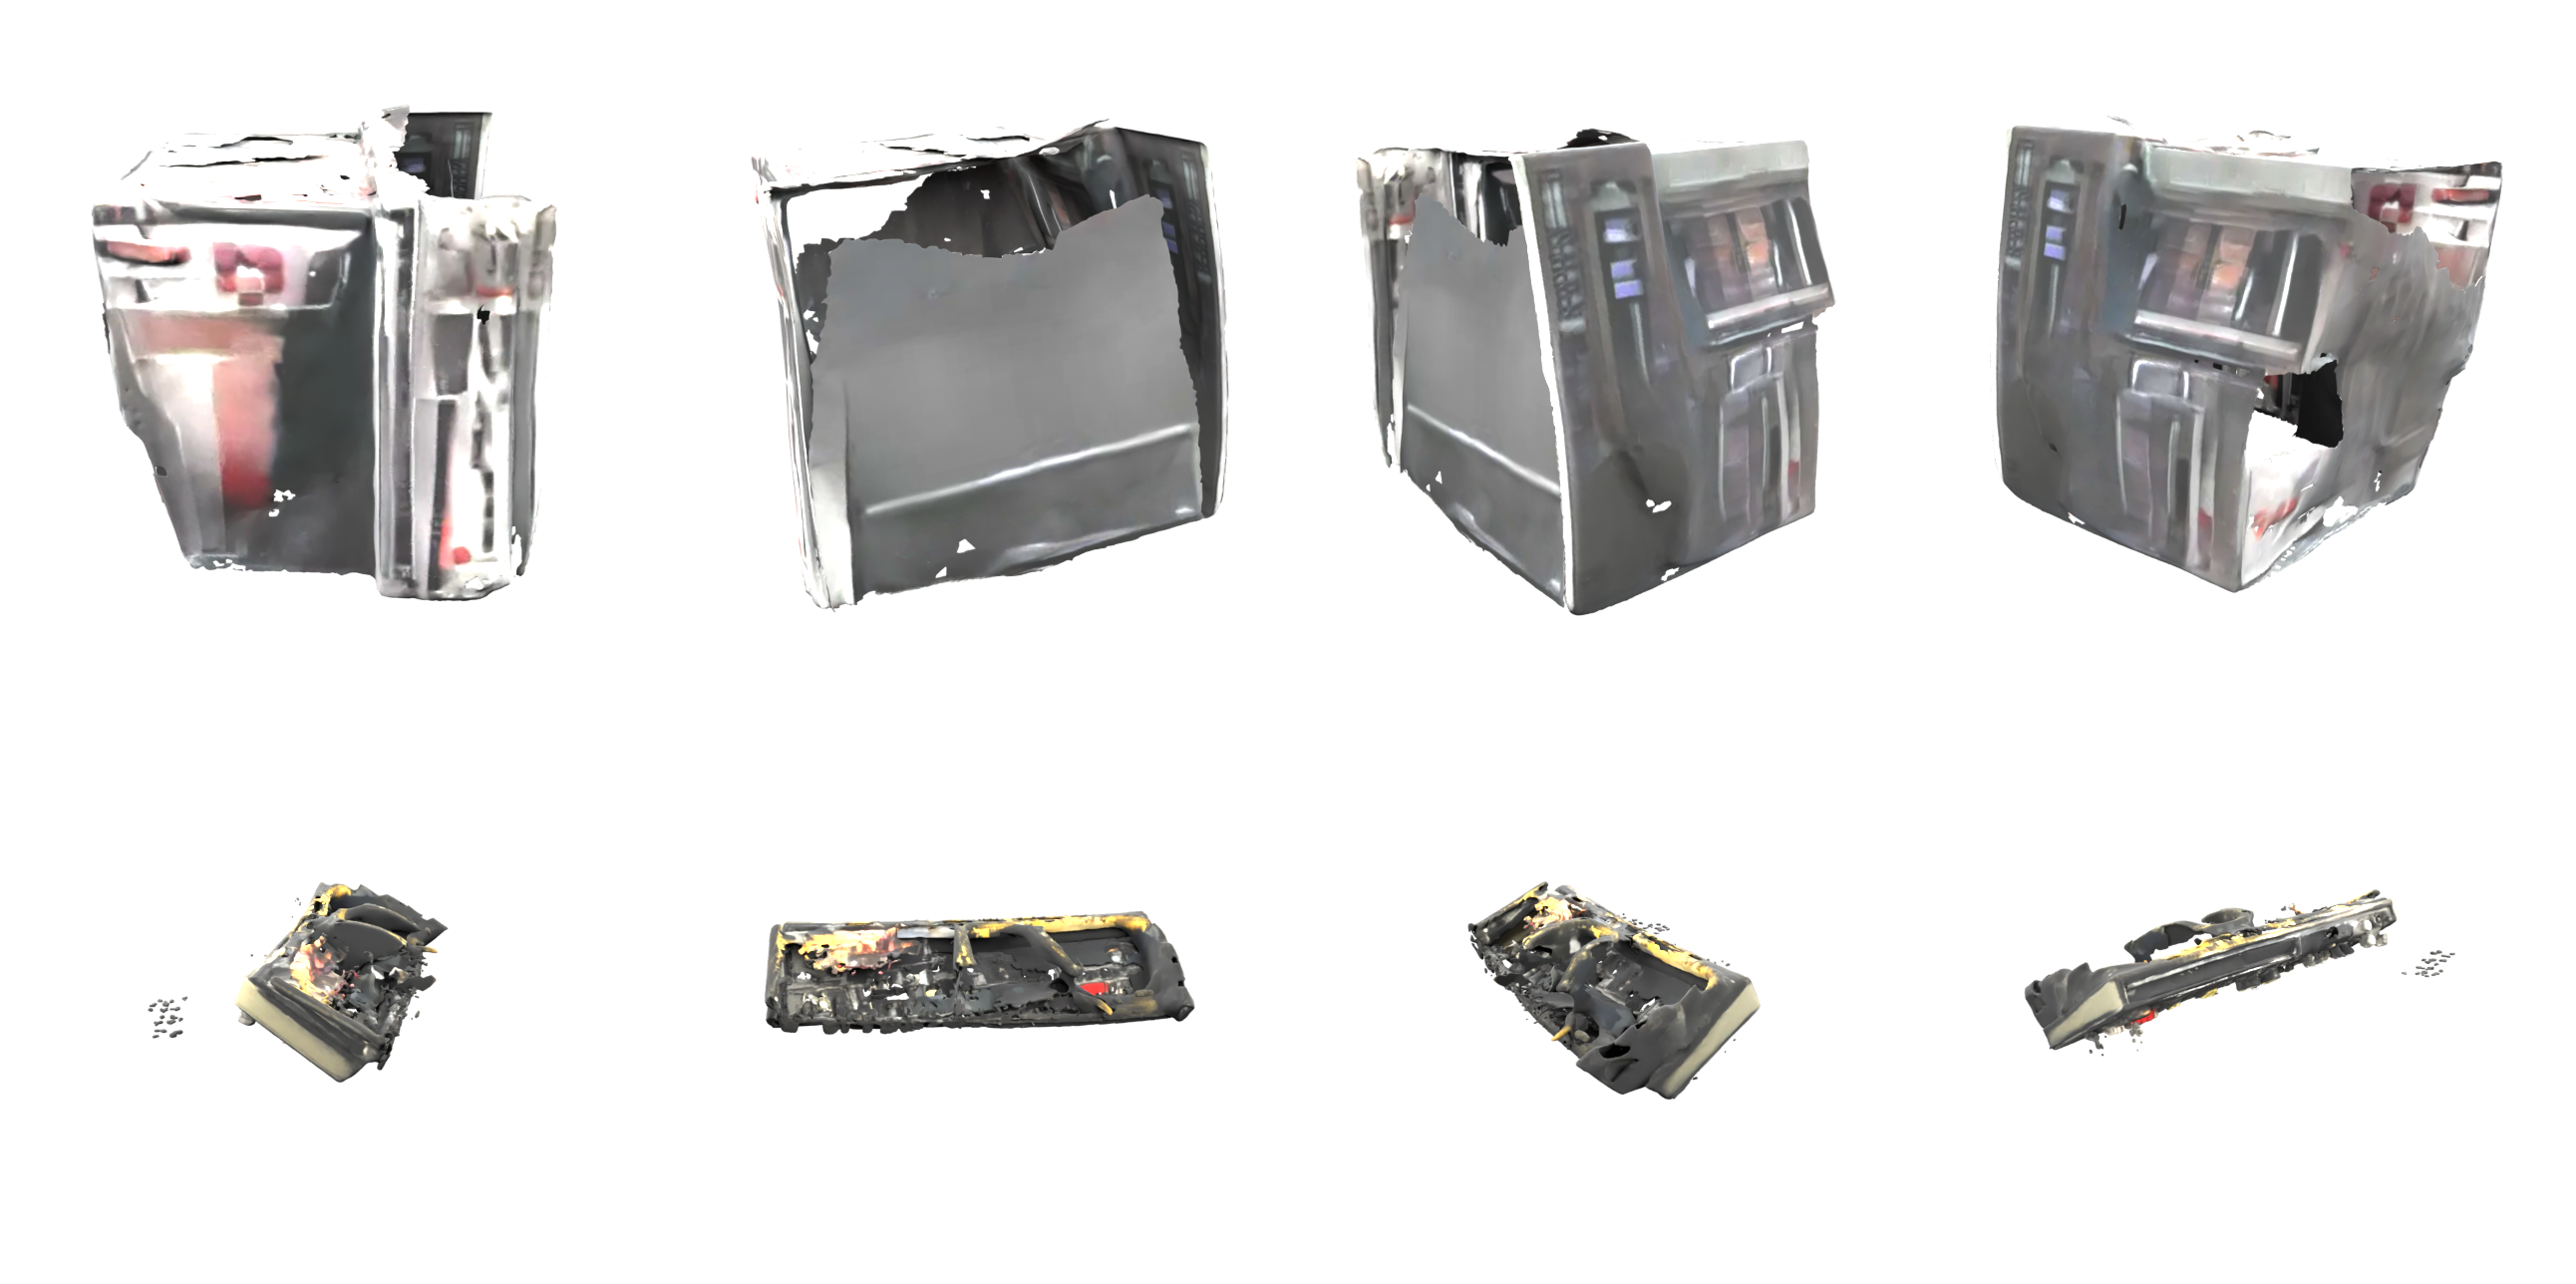
\includegraphics[width=0.98\textwidth]{renders/radio_bakeoff_AvB.png}
\caption{The radio reconstructed by Lane~A (TRELLIS.2 single crop, top) and Lane~B (ReconViaGen
multi-view, bottom), same four viewpoints. Observations only: Lane~A yields a closed, continuous
housing with soft surface detail; Lane~B yields separated front-panel components with visible
floaters and thin shells. No quality ranking is implied --- numeric silhouette scoring is deferred
(\S\ref{sec:eval-ranking}).}
\label{fig:bakeoffvisual}
\end{figure*}

Quality ranking across lanes is deferred: the nc04 numeric silhouette scores are not yet
reliable (the scale bracket was only just fixed via the manifest \texttt{scene\_scale}, and refined
scoring is running), so visual contact sheets are the current evidence and no numeric lane winner is
claimed. The ranking chart lands when refined scoring completes (\S\ref{sec:eval-ranking}).

% SRC: VALIDATION.md §3-4; DESIGN.md validation; ADR-002 fairness
\section{Evaluation}

Evaluation is observed-vs-withheld throughout. A held-out azimuth sector (25\% of views
on the gallery set) is never merged into observed metrics, so backside quality cannot be inflated by
front-face coverage. % SRC: runs/gallery-object-eval/validation.json + summary.json (metrics, GT counts)
Three metric families run: 3D F1 and IoU by voxel-occupancy overlap of carved
Gaussian centres against the best-matching ground-truth cloud (voxel = 1\% scene scale = 0.123);
reproj-IoU, a coarse point-splat silhouette reprojected into each camera against the SAM mask; and
mesh sanity (component count, watertightness, non-manifold edges) run on the reference mesh as a
baseline for scoring generated meshes later. The ground-truth \texttt{full\_scene.glb} is itself
messy (11{,}583 verts, 356 components, not watertight, 654 non-manifold edges), which is a
useful yardstick.

Two limits qualify the current numbers, both recorded plainly. The reproj-IoU is a lower bound
because there is no true rasteriser: a coarse splat silhouette muddies both the absolute IoU and the
observed/withheld gap, which at this coverage is small and noisy (sometimes withheld exceeds
observed). A real gsplat rasteriser would sharpen both. And the golden set may encode the old
pipeline's assumptions, so it is used for golden regression tests only; a blinded fresh capture with
withheld angular sectors is the true backside benchmark.

Fairness rules for the lane bake-off (from adversarial review) are common mask and frame-selection
inputs, identical finishing and eval, and both fixed-candidate-count and fixed-GPU-time comparisons
with seed variance reported --- not just winners. Candidate selection runs at $512^3$/$1024^3$ and
the winner is regenerated at ship quality.

\subsection{Charts}
One plot shows the over-merge (Figure~\ref{fig:overmerge}). Every marker is a carved object
scored against its best-matching ground-truth cloud; area is the carved Gaussian count. Three
over-merged blobs ($\geq$1M Gaussians) sit top-left: high reproj-IoU because they cover the frame,
low 3D-F1 because they are not one object, while the smaller clean components reach higher F1 to
the right. The lane bake-off chart fills once Lane-A/B runs land.

\begin{figure}[h]
\centering
% SRC: runs/gallery-object-eval/validation.json via scripts/make_closeout_charts.py
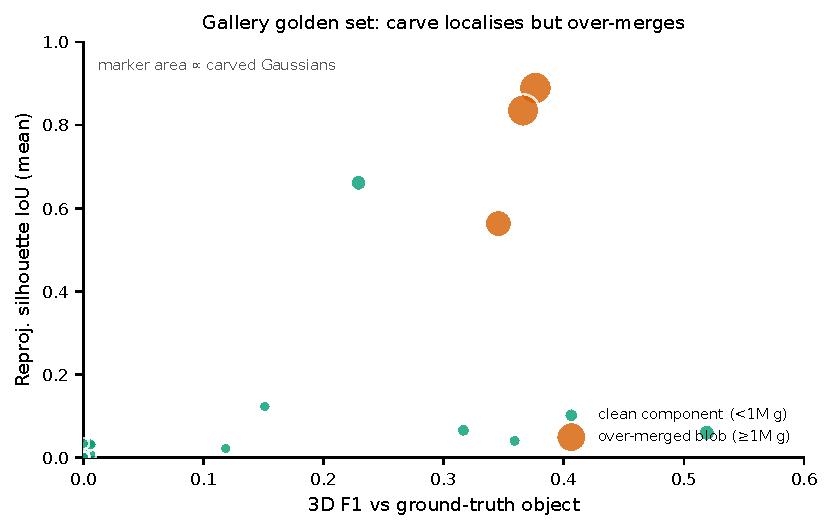
\includegraphics[width=\columnwidth]{gallery-object-eval/charts/gallery_f1_vs_reproj.pdf}
\caption{Carve localises but over-merges where a class tiles the scene.
Marker area $\propto$ carved Gaussians.}
\label{fig:overmerge}
\end{figure}

Resource cost across the bake-off is settled (Figure~\ref{fig:bakeoff}, \S\ref{sec:objgen}):
every Lane-A and Lane-B variant stayed under 32\,GB reserved on Linux/Ada. Quality ranking is not, and the reason is
diagnosed.\label{sec:eval-ranking} % SRC: measured from runs/nc04-object-pass2/objects/radio_00.ply (raw extent) + summary.json scene_scale
The numeric silhouette scores stay low regardless of the
scale/translation search because the pass-2 radio Gaussian subset spans $120.9\times44.1\times125.1$
units in a scene of scale 9.2 --- about $13\times$ the whole scene --- so the per-object carve has
leaked wall and floor into the object (the manifest's robust p5--p95 extent, $15.8\times3.1\times10.7$,
understates it; the true radio core is $\approx$1.5 units). The emplacement anchor (centroid and extent) is therefore unreliable, so absolute
silhouette IoU cannot be trusted as a lane discriminator. This is an upstream carve/mask-sparsity
problem, not a generator or placement bug: generation quality (the turntables, Figure~\ref{fig:turntables})
is the clean signal, while placement precision awaits a cleaner carve. The per-camera contact sheet
(Figure~\ref{fig:contact}) shows the consequence directly --- the candidate silhouette spills beyond
the object on several views. The contact sheets are the evidence of record
and no numeric lane winner is claimed. Since that measurement, the carve leak's root cause was found
and fixed: the automatic depth band was inflated by outlier Gaussians, and a robust p5--p95 band
(commit \texttt{ec4560e}) re-carves the radio to a clean 2{,}093-Gaussian cluster of extent
$0.44\times0.49\times0.46$ units --- a plausible object core in a scene of scale 9.2.
% SRC: runs/nc04-generate-pass1/recarve_score.log (CLEAN_CARVE line)
The degenerate zeros were subsequently traced to view selection, not projection: the scene holds
six radio instances, and the scorer had sampled masks across all of them. Selecting the 24 views that
genuinely observe \texttt{radio\_00} by reprojection overlap (top overlap 0.94) and re-scoring the
three candidates by 7-DoF silhouette alignment against ten of those real cameras gives the first
numeric ranking (Figure~\ref{fig:ranking}): Lane~A (TRELLIS.2 single-crop) 0.212, Lane~B multi-view
0.136, Lane~B single-view 0.127.
% SRC: runs/nc04-generate-pass1/radio_bakeoff_clean.json (BAKEOFF_CLEAN)
The absolute values are moderate --- the anchor extents come from the carved subset and the
rasterisation is silhouette-only --- so the ranking is read as relative evidence on one object, not a
general verdict; it agrees with the visual comparison and completes the previously open ranking item.

\begin{figure}[h]
\centering
% SRC: runs/nc04-generate-pass1/charts/quality_ranking.pdf
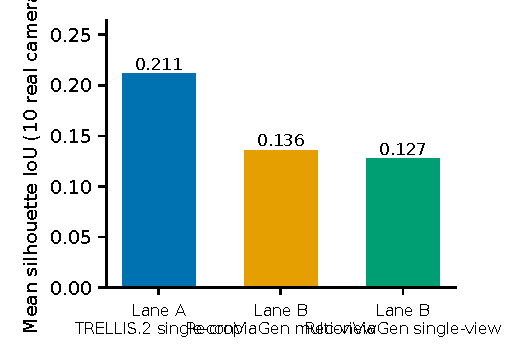
\includegraphics[width=0.85\columnwidth]{quality_ranking.pdf}
\caption{Radio bake-off, numeric ranking: mean silhouette IoU of each candidate against ten real
cameras that observe this instance, after 7-DoF alignment. Lane~A leads; values are relative
evidence for this object rather than a general lane verdict.}
\label{fig:ranking}
\end{figure}

\begin{figure}[h]
\centering
% SRC: runs/nc04-generate-pass1/radio/bakeoff_contact_sheets/radio_laneA_best.png (sidecar select stage)
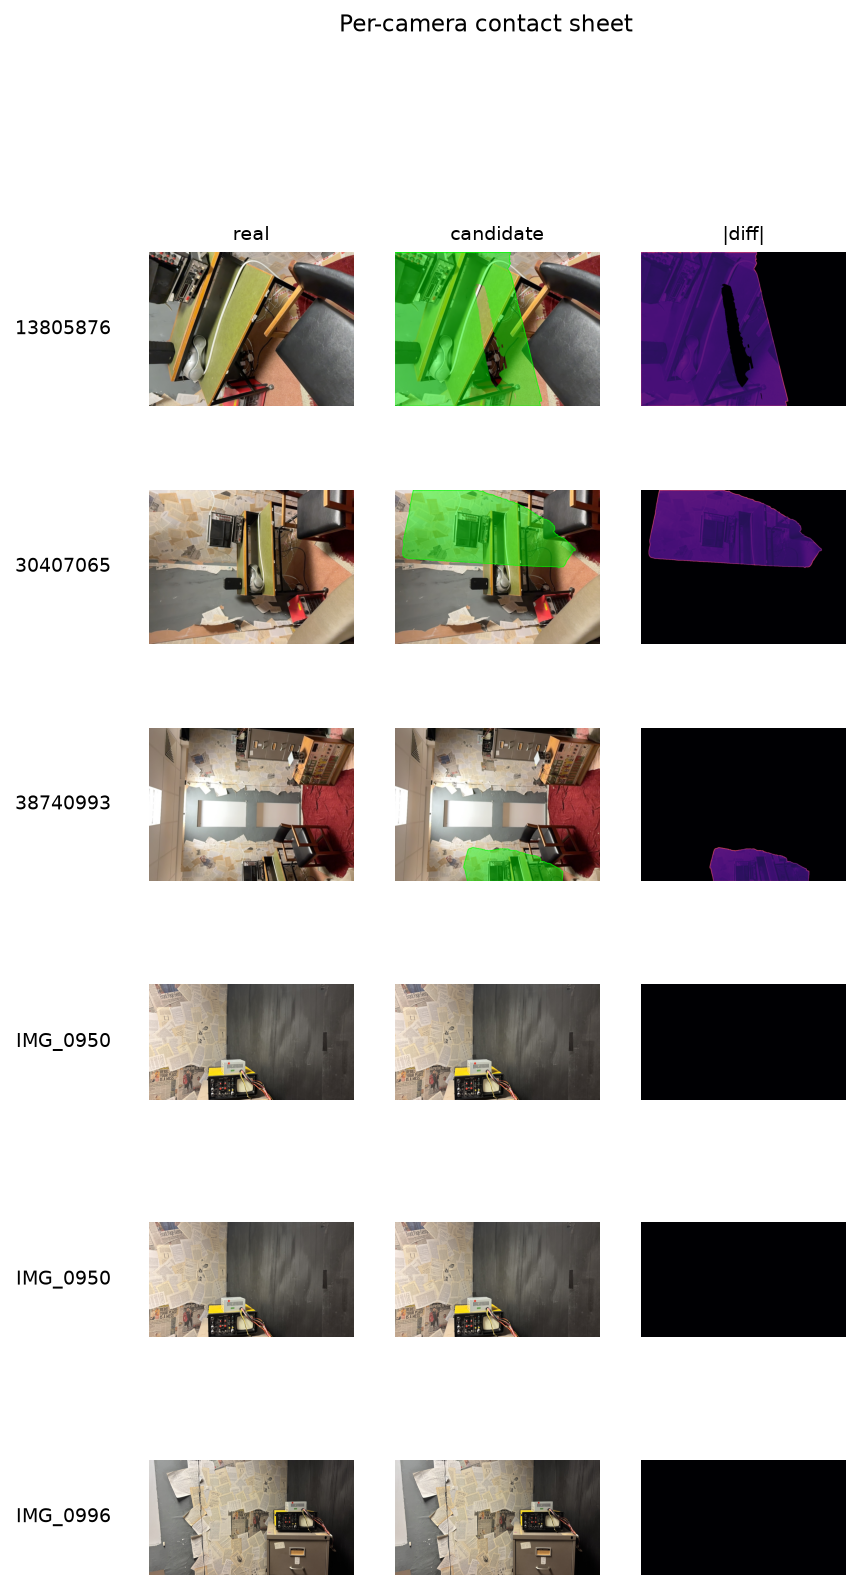
\includegraphics[width=\columnwidth]{renders/contact_radio_laneA.png}
\caption{Per-camera evidence for the Lane-A radio: real frame, candidate silhouette (green) and
absolute difference, across six real cameras. Where the green spills onto walls and furniture the
carve has over-captured, which is why absolute silhouette IoU is not yet a reliable lane score.}
\label{fig:contact}
\end{figure}

% SRC: report.md §7.5-7.7; ADR-001; DESIGN.md "uos-vitrine PR"; VALIDATION.md §1-2
\section{Interface contract and the UoS PR}

Data crosses the boundary as files, not imports. UoS exports a versioned handoff containing the
authoritative scene-PLY hash, the registered staged images, the COLMAP text model, capture metadata,
the coordinate convention, the parent archive-manifest hash and stable object requests. The sidecar
validates the handoff and bypasses its own ingest, SfM and scene retraining. The original full-scene
PLY stays byte-identical and authoritative; a cleaned derivative \texttt{scene\_cleaned.ply} may be
produced by subtracting the exact union of accepted object selections, preserving selection indices,
thresholds and before/after counts, with no inferred background fill by default. Cleaned scene and
generated objects are engine derivatives linked to the master, not replacements for it.

The UoS-side change is kept minimal and additive. \texttt{package.py} gains an optional
\texttt{objects} manifest key and copies \texttt{runs/<name>/objects/} into
\texttt{archive/derivatives/objects/}. \texttt{cli.py} gains a \texttt{vitrine objects} subcommand
that invokes the sidecar as a subprocess. \texttt{serve.py} gains an optional read-only objects
panel. No scene-mesh wiring ships in v1. The integration seam already exists and stands up: the
sidecar venv imports uos-vitrine cleanly and the CLI exposes
\texttt{doctor/\allowbreak ingest/\allowbreak sfm/\allowbreak train/\allowbreak package/\allowbreak objects/\allowbreak evaluate/\allowbreak verify/\allowbreak run}, with \texttt{objects} already
shelling out to the sidecar.

Validation surfaced one real cross-platform defect. \texttt{vitrine verify nested-cinema-04}
re-checksums the manifest but rejects every file: the package was authored on Windows and
\texttt{manifest.json} stores \texttt{originals\textbackslash <name>.jpg} with backslash separators,
which the POSIX path-safety guard flags as an unsafe path. The packager should emit POSIX
separators, or \texttt{verify} should normalise them before the safety check. This is filed for the
UoS PR. Two pull requests are open against the UoS repository:
\href{https://github.com/ArtechShadow/UOS-Vitrine/pull/1}{PR~\#1} (the sidecar hook: the
\texttt{objects} subcommand and manifest key, three commits, 62 tests) and
\href{https://github.com/ArtechShadow/UOS-Vitrine/pull/2}{PR~\#2} (an additive
\texttt{composed\_scene} manifest field, stacked on PR~\#1).

% SRC: models-lane2/STATUS.md licence tables + blockers; ADR-002; DESIGN.md deployment envelope
\section{Licence and deployment envelope}
\label{sec:licence}

The shipped configuration must fit the UoS target: Windows 11, RTX 5090, \SI{32}{\giga\byte} VRAM,
sm\_120 (Blackwell). Development and validation ran on 48\,GB RTX 6000 Ada cards. Per-stage VRAM
peaks are to be measured under an enforced 32\,GB ceiling before any config is declared 5090-fit,
and a real Windows/5090 acceptance run is the release gate. If that run cannot be executed from the
development container, it is recorded as an explicit release blocker rather than hand-waved.
\todo{Windows/5090 acceptance run on real hardware: this remains the release gate.} The measured
evidence so far is under budget on every path. The object pass's instrumented stage (identify)
peaked at \SI{6.6}{\giga\byte} (Figure~\ref{fig:vram}); generation reserved at most
\SI{9.1}{\giga\byte} on Lane~A and \SI{16.6}{\giga\byte} on Lane~B (Figure~\ref{fig:bakeoff}). All
clear the 32\,GB ceiling, Lane~A with roughly $3.5\times$ headroom, so the acceptance run is
expected to confirm rather than discover the envelope.

\begin{figure}[h]
\centering
% SRC: runs/nc04-object-pass1/summary.json via scripts/make_closeout_charts.py
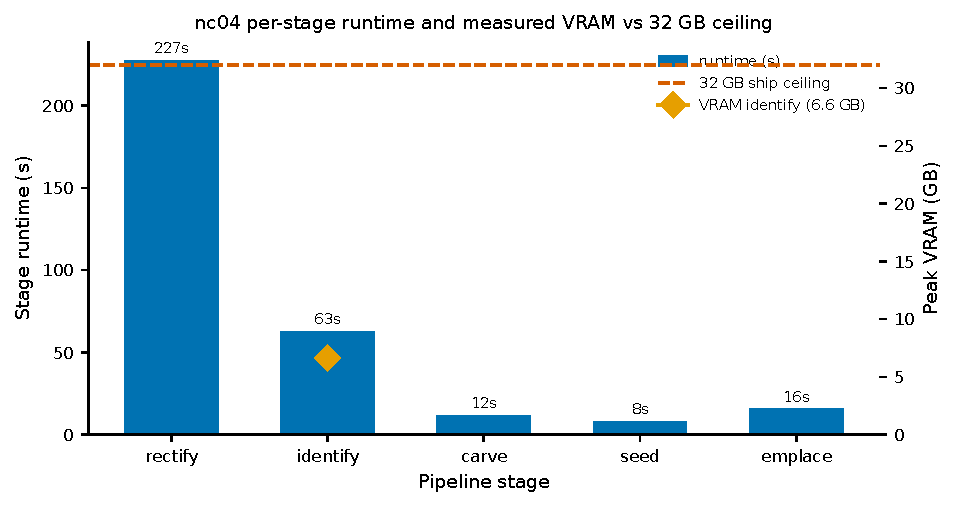
\includegraphics[width=\columnwidth]{nc04-object-pass1/charts/vram_runtime.pdf}
\caption{nc04 per-stage runtime with the measured VRAM peak against the 32\,GB ship ceiling.
Only \texttt{identify} was VRAM-instrumented in pass~1; the others are marked as unmeasured
rather than assumed.}
\label{fig:vram}
\end{figure}

Licence gating decides what can ship. Table~\ref{tab:licence} reproduces the audited findings. The
decisive point: ReconViaGen v0.5 does not load the Facebook VGGT checkpoint --- it loads
\texttt{Stable-X/vggt-object-v0-1}, a VGGT-architecture derivative with \emph{no declared licence},
so a commercial deployment must treat it as encumbered by Meta's VGGT CC-BY-NC terms until clarified.
The plain VGGT arm loads \texttt{facebook/VGGT-1B} (CC-BY-NC, research/eval only); its commercial
checkpoint is gated behind a manual application form and was not accepted on the owner's behalf.
Consequently \textbf{Lane~B is research/eval-only for this closeout} unless the commercial checkpoint
is obtained. Lane~A (TRELLIS.2-4B, MIT) and everything else in the finishing path are clean. Every
checkpoint used is recorded in lineage: repo, commit, hash and licence class.

\begin{table}[t]
\centering\small
\caption{Model licence gate (audited 2026-08-28).
% SRC: models-lane2/STATUS.md; ADR-002 gate table
}
\label{tab:licence}
\setlength{\tabcolsep}{3pt}
\begin{tabular}{@{}p{0.40\columnwidth}p{0.30\columnwidth}p{0.20\columnwidth}@{}}
\toprule
Component & Licence & Gate \\
\midrule
ReconViaGen v0.5 code & MIT & clean \\
microsoft/TRELLIS.2-4B & MIT & clean \\
Stable-X/trellis-vggt-v0-2 & MIT & clean \\
Stable-X/vggt-object-v0-1 & none declared & treat as NC \\
facebook/VGGT-1B & CC-BY-NC-4.0 & eval only \\
facebook/VGGT-1B-Commercial & gated form & not accepted \\
Hunyuan3D-2.1 & Tencent custom & review before ship \\
SAM3.1 checkpoint (local) & unverified & verify before ship \\
\bottomrule
\end{tabular}
\end{table}

Two environment blockers keep Lane~B unreproduced here. ReconViaGen pins conda py3.10 +
torch 2.4/cu121 with five source-compiled CUDA extensions and cp310 prebuilt wheels
(flash-attn, kaolin, xformers), none installable on the container's nix py3.12; and it ships only a
Gradio demo, so a headless run needs a custom driver written after the environment is solved. The
recommended route is a \texttt{uv}-managed standalone py3.10 in the workspace (mechanism confirmed;
the Docker-via-host-socket route is a documented mount trap). The VGGT arm is fully operational: a
smoke test inferred six gallery frames in \SI{0.94}{\second} at \SI{8.1}{\giga\byte} peak. Lane~A
TRELLIS.2-4B weights (\SI{16}{\giga\byte}) are staged on disk by symlink from a read-only mount, so
no re-download was needed.

% SRC: report.md §5.3, §8; VALIDATION.md §4; nc04-object-pass1/REPORT.md; ADR-002/003
\section{Limitations and negative results}

Recording failure is part of the preservation method. The clearest scene-side negative result is the
archive-profile opacity collapse (\S2): the 1600/4096 workstation-archive profile drives 98.7--99.8\%
of the Gaussian population transparent and is quarantined as unvalidated. Omitting it would create the
false impression that six million Gaussians are inherently superior; reporting the full matrix
constrains future claims and keeps throughput capability distinct from reconstruction quality.

On the object side, carve over-merges where one class tiles the scene. On the gallery golden set,
per-label mask unions collapse wall-to-wall paintings into a few multi-million-Gaussian blobs that
overlap one ground-truth object; individual instances are recovered only as smaller, sometimes
fragmentary components. The fix is per-instance masks fed to carve separately, not per-label unions. % SRC: runs/nc04-object-pass2/objects/radio_00.ply raw extent vs summary.json scene_scale=9.2
 The same fault has a stark scale consequence on nc04. Measured directly, the recovered radio
Gaussian subset (118{,}070 splats) spans $120.9\times44.1\times125.1$ units in a scene of scale 9.2
--- roughly $13\times$ the whole scene, i.e. the per-object carve leaked the entire room into the
object. The manifest's robust p5--p95 extent field ($15.8\times3.1\times10.7$) understates this; the
radio's true core is about 1.5 units (inter-quartile). This upstream carve/mask-sparsity leak, not
any generation or placement defect, is what caps silhouette-refined placement until the carve is
cleaned.
Orientation remains the weakest emplacement axis: placement solves translation and scale from the
carve subset reliably, but full orientation must be recovered from silhouettes and is marked
\texttt{needs\_review} when under-constrained --- low-confidence placements must not be presented as
validated assets, and generated backsides and occluded surfaces are labelled inferred.

Further limits, stated plainly: a splat interpolates views, it does not measure surfaces, and COLMAP recovers
arbitrary scale unless an external measurement establishes world units. Mirrors, screens, glass and
polished metal are represented by observed pixels, not physical optics; moving screens are
constitutive to the artwork and a static splat cannot preserve their temporal sequence. Pass~1 left Camera~5's 4K walkthrough (120 frames) unused because only the \texttt{.MOV} shipped;
pass~2 extracted and used all 120, adding the densest trajectory. GroundingDINO phrase-merging pollutes labels
(``armchair chair'', ``radio typewriter''); it is cosmetic for carve but needs one prompt per detect
call. And the reproj-IoU metric is a lower bound until a real gsplat rasteriser replaces the coarse
point-splat silhouette.

% SRC: report.md §9; VALIDATION.md §5; DESIGN.md; ADR-002/003
\section{Recommendations and handover}

\textbf{Scene pipeline.} Quarantine the 1600/4096 workstation-archive profile and keep the
\SI{25.06}{\decibel} RTX 5090 control as the verified workstation baseline. Do not promote the Q1
candidate --- it stayed healthy but scored lower. Future tuning should vary one axis at a time
(post-densification refinement, multi-crop batches, opacity regularisation) with live-opacity
percentage monitored as an acceptance metric, rejecting runs below a declared health threshold. Run a
stills-only 5090 baseline from the 72 archival masters before requesting any reshoot, and complete the
formal newspaper-legibility and matched-view Luma comparisons using saved cameras rather than a single
subjective orbit.

\textbf{Object pipeline.} The biggest available fix is per-instance masks: feed each detection box's SAM
mask into carve separately so tiling classes do not collapse into one blob. Add a real gsplat
rasteriser for silhouette, PSNR and SSIM to sharpen the observed/withheld gap. Complete the lane
bake-off once Lane~B's environment is stood up via the \texttt{uv} py3.10 route, and resolve the
Stable-X checkpoint licence before any commercial Lane~B ship. Extract Camera~5's walkthrough frames to
add the densest trajectory, and normalise GroundingDINO prompts to one per detect call.

\textbf{Integration and handover.} Land the minimal additive UoS PR (\S6), including the
Windows$\rightarrow$POSIX path normalisation in the packager/verify. Seal the preferred scene package
with originals, COLMAP text model, training report, derivatives and limitations under a stable run
identifier before creating any object or engine derivatives. Preserve stable IDs across masks, crops,
selections, reconstructed assets and placements, and disable cloud fallbacks for preservation runs.
The two repositories stay separate in code, licence, product identity and preservation responsibility;
the file contract is the boundary that keeps them so.

Both UoS PRs are open (sidecar hook \#1, composed-scene field \#2). The remaining gates are the
Windows/5090 acceptance run, the refined-scoring lane winner regenerated at ship quality, PR review
and merge, and the sealed-package hashes. \todo{Tick these off at final handover.}

% SRC: report.md Appendix C; models-lane2/STATUS.md; DESIGN.md
\onecolumn
\section*{Appendix A: environment snapshot}
\addcontentsline{toc}{section}{Appendix A: environment snapshot}
\small

\begin{table}[h]
\centering
\caption{Validated environments. Scene pipeline (UoS) and object sidecar (DreamLab).
% SRC: report.md Appendix C; models-lane2/STATUS.md
}
\begin{tabular}{@{}ll@{}}
\toprule
Component & Validated value \\
\midrule
Scene Python / Torch & 3.11 venv; Torch 2.11, CUDA 12.8 \\
gsplat & 1.5.3 \\
Laptop GPU & RTX 3060 Laptop, 6\,GB, compute 8.6 \\
Workstation GPU & RTX 5090 class, 32\,GB (ship target sm\_120) \\
COLMAP & Docker image \\
Master splat & Full-SH 3DGS PLY; SHA-256 manifest \\
\midrule
Sidecar Python / Torch & nix py3.12; Torch 2.4.0 cu121 (Lane~B venv) \\
Dev GPUs & RTX 6000 Ada (sm\_89) + A6000 (sm\_86), 48\,GB \\
TRELLIS.2-4B weights & 16\,GB, symlinked from read-only mount \\
VGGT smoke & 6 frames, 0.94\,s, 8.1\,GB peak (facebook/VGGT-1B, eval only) \\
Sidecar test suite & 112 passed, 0 failed (not-slow) \\
\bottomrule
\end{tabular}
\end{table}

\section*{Appendix B: preservation package schema}
\addcontentsline{toc}{section}{Appendix B: preservation package schema}
% SRC: report.md Appendix B (lines 486-496)
\begin{verbatim}
archive/
  originals/     untouched camera photographs and video
  sfm/           cameras.txt, images.txt, points3D.txt, database.db
  model/         scene.ply, full spherical harmonics
  derivatives/   web splat, mesh, previews, objects/ (sidecar output)
  manifest.json  versions, settings, metrics, SHA-256 fixity
  README.md      plain-language context and verification instructions
\end{verbatim}
Manifest schema identifier \texttt{vitrine/preservation-package/1}; object records
\texttt{vitrine/object/1}. Verification detects corruption or unintended change; it does not
replace a backup and replication policy.

\section*{Appendix C: ReconViaGen environment blockers}
\addcontentsline{toc}{section}{Appendix C: ReconViaGen environment blockers}
% SRC: models-lane2/STATUS.md §Blockers B1-B3
\begin{itemize}
\item \textbf{B1}: ReconViaGen \texttt{setup.sh} pins conda py3.10 + torch 2.4.0/cu121 with
cp310 prebuilt wheels (flash-attn 2.7.0.post2, kaolin, xformers) and five source-compiled CUDA
extensions (nvdiffrast, nvdiffrec, CuMesh, FlexGEMM, o-voxel); none install on the nix py3.12 venv.
Recommended route: \texttt{uv}-managed standalone py3.10 (mechanism confirmed).
\item \textbf{B2}: v0.5 ships only a Gradio demo (\texttt{app\_v05.py}), no headless CLI; an
automated run needs a custom driver around \texttt{TrellisHybridPipeline} after B1.
\item \textbf{B3}: 256\,MB tmpfs caches hit ENOSPC; resolved by redirecting HF/pip/TMP caches to
the workspace disk.
\end{itemize}


\section*{Appendix D: reproducibility}
\addcontentsline{toc}{section}{Appendix D: reproducibility}
% SRC: git rev-parse (uos-vitrine main, object-sidecar HEAD, PR branches); run REPORTs; scripts
\small

\textbf{Repositories and commits.} UoS Vitrine \texttt{main} at \texttt{0e3f862} (MIT, public).
Object sidecar \texttt{main} at \texttt{6fb288d}. PRs against UoS (all four merged):
\href{https://github.com/ArtechShadow/UOS-Vitrine/pull/1}{\#1}
(\texttt{feature/object-sidecar-hook-clean}) and
\href{https://github.com/ArtechShadow/UOS-Vitrine/pull/2}{\#2}
(\texttt{feature/composed-scene-export}).

\textbf{Hardware matrix.} Dev/validation: RTX 6000 Ada (sm\_89, 48\,GB, GPU2) and A6000 (sm\_86);
driver 610.57.04, CUDA 12.9 runtime; nix Python 3.11/3.12. Ship target (not yet run): Windows 11,
RTX 5090 (sm\_120, 32\,GB).

\textbf{Commands.}
\begin{verbatim}
# object pass (identify->carve->seed->emplace)
cd object-sidecar && source smoke/env.sh
CUDA_VISIBLE_DEVICES=2 .venv/bin/python -m sidecar run \
  --package ../datasets/nested-cinema-04 \
  --out ../runs/nc04-object-pass2 --max-frames 0
# Lane-A generation (TRELLIS.2)
python models-lane2/run_reconviagen.py   # Lane-B (uv py3.10 env)
# charts + turntables
.venv/bin/python scripts/make_closeout_charts.py
blender --background --python scripts/render_turntable.py -- <glb> <out> <stem>
\end{verbatim}

\textbf{Artefact paths.} Scene runs \texttt{runs/nc04-object-pass\{1,2\}/}; generation
\texttt{runs/nc04-generate-pass1/}; Lane-B \texttt{runs/nc04-laneb-pass1/}; golden eval
\texttt{runs/gallery-object-eval/}; charts \texttt{runs/*/charts/}; renders and contact sheets under
\texttt{runs/nc04-generate-pass1/radio/}.

\textbf{Verification.} \texttt{vitrine verify <package>} re-hashes the manifest (note the
Windows-backslash defect, \S6). Sidecar suite: \texttt{pytest -m "not slow"} (112 passed);
UoS PR\#1 adds 62 tests.

\textbf{Open gates at closeout.} Windows 11 / RTX 5090 acceptance run; carve de-contamination and
refined silhouette scoring (then the quality-ranking chart); clean-machine ReconViaGen environment
rebuild and a commercial-eligible checkpoint path; PR review and merge; sealed-package hashes.


\end{document}
